% !TeX root = ../thesis.tex

\chapter{Ansatz}
\label{sec:concepts}
Ein Fahrstreifenwechsel ist ein h\"aufig angewendetes Fahrman\"over das aus verschieden Gr\"unden durchgef\"uhrt wird.
So kann ein Fahrstreifenwechsel notwendig sein um einer vorgegebenen Route zu folgen oder er wird durchgef\"uhrt um ein langsameres Fahrzeug zu \"uberholen.
Da ein Fahrstreifenwechsel von mehreren Verkehrsteilnehmern gleichzeitig abh\"angt ist er ein komplexes Fahrman\"over \cite{Gipps1986}.
Dies gilt vor allem bei dichtem Verkehr.
F\"ur einen erfolgreichen und sicheren Fahrstreifenwechsel in dichtem Verkehr sind sowohl taktische Entscheidungen (\cite{Ulbrich2015towards}) als auch ein kooperatives Verhalten (\cite{Wei2013}) notwendig.

In diesem Kapitel wird ein Ansatz f\"ur die Trajektorienplanung eines kooperativen Fahrstreifenwechsel von hochautomatisierten Fahrzeugen vorgestellt.
Der Fahrstreifenwechsel findet in Interaktion mit nicht automatisierten Fahrzeugen statt.
Dazu soll zun\"achst die Auswahl des Basisalgorithmus begr\"undet werden.
In diesem Zuge wird auf einige Grundlagen zum Thema Fahrstreifenwechsel eingegangen.
Anschlie{\ss}end werden die Einschr\"ankungen, die sich durch den Basisalgorithmus ergeben, beschrieben.
Aus den Einschr\"ankungen l\"asst sich ableiten welche Anpassungen des Basisalgorithmus f\"ur die Anwendung bei einen Fahrstreifenwechsel notwendig sind.
Basierend darauf wird der Ansatz f\"ur einen einzelnen Planungsschritt vorgestellt.
Aufgrund von Unsicherheiten unterschiedlicher Art in der Planung muss dieser Planungsschritt in regelm\"a{\ss}igen zeitlichen Abst\"anden wiederholt werden.
Auf diesen Aspekt wird in Kapitel~\ref{sec:Neuplanung} eingegangen.

\section{Auswahl und Einschr\"ankungen des Basisalgorithmus}
In diesem Abschnitt wird zun\"achst die Auswahl Basisalgorithmus begr\"undet.
In dieser Arbeit wurde der von Naumann und Stiller \cite{Naumann2017towards} vorgestellte Ansatz f\"ur eine kooperative Bewegungsplanung als Basisalgorithmus ausgw\"ahlt. 
Zur Begr\"undung der Auswahl wird auf einige grundlegende Aspekte eines Fahrstreifenwechsels eingegangen.
Aus dem Basisalgorithmus ergeben sich Einschr\"ankungen die daf\"ur sorgen, dass er nicht direkt auf einen Fahrstreifenwechsel anwendbar ist.
Diese sollen anschlie{\ss}end herrausgearbeitet werden.
Aus den sich ergebenden Einschr\"ankungen l\"asst sich schlie{\ss}en, welche Anpassungen notwendig sind um den Ansatz der kooperativen Bewegungsplanung auf eine Fahrstreifenwechsel anzuwenden. 

\subsection{Auswahl des Basisalgorithmus}
\label{sec:AuswahlBA}
Fahrstreifenwechsel sind gebr\"auchliche Fahrman\"over in allt\"aglichen Fahrsituationen.
Die Gr\"unde aus denen ein Fahrstreifenwechsel ausgef\"uhrt wird sind unterscheidlich.
In der Literatur wird h\"aufig zwischen zwingend notwendigen (englisch: mandatory) und frei verf\"ugbaren (englisch: discretionary) Fahrstreifenwechseln unterschieden (\cite{Toledo2003}, \cite{Yang1996}).
Ein Fahrstreifenwechsel ist zwingend notwendig, wenn der aktuelle Fahrstreifen endet oder um einer vorgegebenen Route zu folgen.
Frei verf\"ugbare Fahrstreifenwechsel werden in erster Linie angewandt um langsamere Fahrzeuge zu \"uberholen.

Ein Fahrstreifenwechsel stellt ein vergleichsweise komplexes Fahrman\"over dar, das gro{\ss}es Potential f\"ur Sicherheitsrisiken birgt und direkten Einfluss auf den Verkehrsfluss hat \cite{Julian2015}.
Bei dichtem Verkehr muss in der Planung die Interaktion mit anderen Fahrzeugen ber\"ucksichtigt werden \cite{Hubmann2018}.
Es muss ein Kompromiss zwischen den eigenen Vorteilen und den Nachteilen anderer Verkehrsteilnehmer gefunden werden \cite{Kesting2007}.
Laut Gipps \cite{Gipps1986} m\"ussen folgende taktische Entscheidungen getroffen werden: 

\begin{itemize}
\item Ist ein Fahrstreifenwechsel m\"oglich
\item Ist ein Fahrstreifenwechsel notwendig
\item Ist ein Fahrstreifenwechsel w\"unschenswert
\end{itemize}


Viele existierende Ans\"atze unterteilen das Planungsproblem f\"ur einen Fahrstreifenwechsel in mehrere Teilprobleme. 
Zu den Teilproblemen geh\"ort die L\"uckenauswahl, die Ann\"aherung an die L\"ucke, die Bewertung der L\"ucke und das Einf\"adeln in die L\"ucke.
Diese Teilprobleme werden getrennt voneinander gel\"ost. \cite{Hubmann2018}
Laut Hubmann et al. \cite{Hubmann2018} ist dadurch zwar eine vereinfachte, hierachische Problemformulierung m\"oglich, es wird jedoch gleichzeitig der Raum m\"oglicher L\"osung reduziert.
Dies kann dazu f\"uhren, dass bei dichtem Verkehr keine L\"osung gefunden werden kann.
Handelt es sich um einen notwendigen Fahrstreifenwechsel bedeutet dies, dass das Fahrzeug auf dem aktuellen Fahrstreifen zum Stehen kommt bis sich eine L\"ucke bietet, die gro{\ss} genug ist, um den Fahrstreifenwechsel sicher ausf\"uhren zu k\"onnen.
Dies erschwert den Fahrstreifenwechsel noch weiter und birgt au{\ss}erdem hohe Sicherheitsrisiken und sollte deshalb m\"oglichst vermieden werden.

Menschlich gef\"uhrten Fahrzeugen gelingt ein Fahrstreifenwechsel in der Regel auch in dichtem Verkehr.
Dies liegt dran, dass sie in vielen F\"allen sowohl kooperatives Verhalten gegen\"uber anderen Fahrzeuge zeigen als auch kooperatives Verhalten von anderen Fahrzeugen erwarten.
Ein solches Verhalten ist m\"oglich, weil Menschen in der Regel die Intentionen anderer Fahrzeuge einsch\"atzen k\"onnen und entsprechend darauf reagieren.
Bei einem Fahrstreifenwechsel k\"onnen die Fahrzeuge auf dem Zielfahrstreifen auf unterschiedliche Arten ein kooperatives Verhalten zeigen.
Sie k\"onnen ihre Geschwindigkeit leicht erh\"ohen oder verringern um die L\"ucke f\"ur das auffahrende Fahrzeuge zu vergr\"o{\ss}ern.
Oder sie machen ebenfalls einen Fahrstreifenwechsel auf einen dritten Fahrstreifen und machen so eine L\"ucke auf dem Zielfahrstreifen des Ego"=Fahrzeuges auf.
Automatisierte Fahrzeug, die nicht \"uber ein kooperatives Verhalten verf\"ugen, zeigen in solchen Situationen h\"aufig ein Verhalten das als sozial nicht akzeptabel beschrieben werden kann.
Das f\"uhrt dazu, dass es f\"ur menschliche Fahrer schwer wird automatisierte Fahrzeuge einzusch\"atzen und k\"onnte zu gef\"ahrlichen Situationen f\"uhren. \cite{Wei2013}

Aus diesem Grund sollten f\"ur einen Fahrstreifenwechsel bei dichtem Verkehr ein kooperativer Planungsansatz mit interaktionsbewusster Bewegungspr\"adiktion verwendet werden.
In Wei et al. \cite{Wei2013} konnte durch einen Ansatz der ein soziales, kooperatives Fahrverhalten ber\"ucksichtigt die Kosten f\"ur einen Fahrstreifenwechsel um 41.7 \% reduziert werden.
Der Vergleich fand aufgrund eines ausgew\"ahlten Kostenfunktionals statt.
Eine Planung in der die Interaktion mit anderen Fahrzeugen ber\"ucksichtigt wird f\"uhrt jedoch dazu, dass die Bewegungspr\"adiktion anderer Fahrzeuge nicht mehr entkoppelt von der Trajektorienplanung stattfinden kann \cite{Hubmann2018}.
Es muss also ein Ansatz gew\"ahlt werden, bei der die Bewegungspr\"aditktion in die Bewegungsplanung integriert wird.

Diese M\"oglichkeit bietet der von Naumann und Stiller \cite{Naumann2017towards} vorgestellte Ansatz einer Mulit"=Agenten"=Optimierung.
Durch die Verwendung eines Kostenfunktionals, das die Gesamtkosten aller Fahrzeuge ber\"ucksichtigt, wird von einem kooperativen Verhalten aller Fahrzeuge ausgegangen.
Der Ansatz bietet au{\ss}erdem die M\"oglichkeit ebenfalls die Man\"overplanung in die Bewegungsplanung zu integrieren.
Er wurde deshalb als Basisalgorithmus ausgew\"ahlt.
Es ergeben sich jedoch Einschr\"ankungen die eine Anpassung f\"ur die Anwendung auf einen Fahrstreifenwechsel notwendig machen.
Diese werden im n\"achsten Abschnitt erl\"autert.


\subsection{Einschr\"ankungen des Basisalgorithums}
\label{Grenzen}
Der von Naumann und Stiller \cite{Naumann2017towards} vorgestellte Ansatz zur kooperativen Trajektorienplanung, der hier als Basisalgorithmus bezeichnet wird, wurde bereits simulativ in zwei Verkehrszenarien validiert.
Diese zwei Verkehrszenarien stellen zwei typische Situationen dar, in den \"ublicherweise kooperatives Verhalten gefordert ist.
In einer ersten Simulation wurde der Ansatz f\"ur eine Trajektorienplanung an einer ungeregelten Engstelle (siehe Abbildung~\ref{fig:Engstelle}) validiert.
Hier steht zwei entgegengerichteten Fahrrichtungen f\"ur einen kurzen Abschnitt lediglich eine gemeinsame Spur zur Verf\"ugung.
Die Fahrzeuge m\"ussen entscheiden welches zuerst in die Engstelle einf\"ahrt und welches das andere Fahrzeug passieren lassen muss.
Bei einem rein reaktiven Ansatz bei dem beide Fahrzeuge davon ausgehen, dass das jeweils anderen Fahrzeug zuerst einf\"ahrt, kann dies zu einer Patt"=Situationen f\"uhren in der beide Fahrzeuge zum Stillstand kommen.
In einem zweiten Szenario wurde das Linksabbiegen an einer T-Kreuzung simuliert (siehe Abbildung~\ref{fig:Kreuzung}).
In dieser Situation muss das Ego"=Fahrzeug aufgrund des Kostenfunktionals entscheiden, ob es vor oder nach dem entgegenkommenden Fahrzeug abbiegen soll.
Die beiden Szenarien sind in Abbildung~\ref{fig:SimSzen} dargestellt.

\begin{figure}[!htbp]
    \centering
    \subfigure[Engstelle ohne Vorfahrtsregelung \cite{Naumann2017towards}]{
        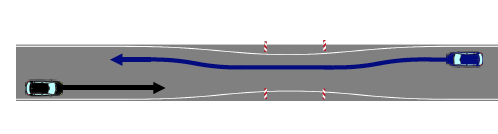
\includegraphics[width = 0.55 \textwidth]{Engstelle.png}
        \label{fig:Engstelle}
    }
    \hfill
     %add desired spacing between images, e. g. ~, \quad, \qquad, \hfill etc.
     %(or a blank line to force the subfigure onto a new line)
    \subfigure[Linksabbiegen an einer T-Kreuzung  \cite{Naumann2017towards}]{
        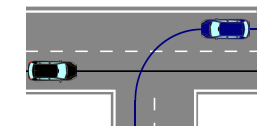
\includegraphics[width = 0.35  \textwidth]{Kreuzung.png}
        \label{fig:Kreuzung}
    }
    \caption[Anpassung f\"ur globales Minimum]{Simulierte Szenarien des Basisalgorithmus}
    \label{fig:SimSzen}
\end{figure}

Anhand der Simulationen konnte gezeigt werden, dass es dem Ansatz des Basisalgotihmus in beiden Szenarien m\"oglich ist sichere, komfortabel und kooperative Trajektorien zu generieren.
Auch ohne eine sogenannte Fahrzeug"=zu"=Fahrzeug Kommunikation konnte mit anderen Fahrzeugen kooperiert werden und damit eine vorteilhafte L\"osung gefunden werden.
In beiden F\"allen konnten die Pfade der beteiligten Fahrzeuge als durch den Streckenverlauf gegeben angenommen werden.
Zur Generierung von m\"oglichen Trajektorien mussten deshalb nur noch verschiedene Geschwindigkeitsprofile erzeugt werden.
Die in Kapitel~\ref{sec:SmapPVD} beschriebene Path"=Velocity"=Decomposition \gls{pvd} ist somit direkt anwendbar.
F\"ur beide Fahrzeuge wurde nun eine Vielzahl von zuf\"alligen Trajektorien generiert und anschlie{\ss}end alle sich ergebenden Kombinationen anhand eines Kostenfunktionals bewertet.

Wird nun ein Fahrstreifenwechsel betrachtet werden die Einschr\"ankungen des Basisalgorithmus offensichtlich.
Zum einen ist der Pfad bei einem Fahrstreifenwechsel nicht mehr komplett durch den Stra{\ss}enverlauf vorgegeben.
In vielen F\"allen ist nicht vorgegeben wann bzw. wo der Fahrstreifenwechsel eingeleitet werden soll.
Bei einem \"Uberholman\"over auf einer mehrspurigen Fahrbahn sollte der Fahrstreifenwechsel zum \"Uberholen eines langsameren Fahrzeuges eingeleitet werden bevor es zu Unterschreitung von Sicherheitsabst\"anden kommt.
Auf einer Beschleunigungsspur sollte der Fahrstreifenwechsel eingeleitet werden sobald sich eine L\"ucke ergibt die gro{\ss} genug ist.
Der zu fahrende Pfad h\"angt damit stark vom Geschwindigkeitsprofil des Fahrzeuges ab.
Die Ermittlung von Pfad und Geschwindigkeitsprofil kann also nicht entkoppelt voneinander stattfinden.
Ein Ausnahme bilden Einf\"adelszenarien bei denen sich die Fahrzeuge nach dem Rei{\ss}verschlussverfahren auf dem neuen Fahrstreifen einordnen sollen.
Hier ist vorgegeben, dass der Fahrstreifenwechsel am Fahrstreifenende stattfinden soll.
Doch auch hier h\"angt der geometrische Pfad des Fahrstreifenwechsels von der Geschwindigkeit des Fahrzeuges ab.
F\"ahrt das Fahrzeug vergleichsweise langsam, so kann der Fahrstreifenwechsel auf einer relativ kurzen Strecke statt finden.
Bei h\"oheren Geschwindigkeiten w\"urden bei dem selben Pfad die Kr\"ummung des Pfades zu hohen Querbeschleunigungen f\"uhren.
Der Fahrstreifenwechsel muss also auf einer l\"angeren Strecke stattfinden.
Die vorgestellte \gls{pvd} ist somit nicht mehr direkt anwendbar.
Es gilt den Pfad in Abh\"angigkeit vom eigenen Geschwindigkeitsprofil zu generieren.
Gegebenenfalls sollten bei der Pfadplanung auch dynamische Hindernisse, mit denen keine direkte Interaktion stattfindet, in Betracht gezogen werden.

Ein weiterer Nachteil ist, dass der Rechenaufwand f\"ur einen einzelnen Planungsschritt stark von der Anzahl der in Betracht gezogenen Fahrzeuge abh\"angt.
Nehmen wir ein Szenario an, in dem lediglich ein anderes Fahrzeug f\"ur eine Kooperation in Frage kommt.
Dies ist in den beiden simulierten Szenarien der Fall.
Au{\ss}erdem sollen f\"ur jedes der Fahrzeuge 1000 Trajektorien generiert werden.
So ergeben sich \( 10^6 \) m\"ogliche Trajektorienkombinationen.
Kommt ein weiteres Fahrzeug hinzu ergeben sich bereits \( 10^9 \) m\"ogliche Trajektorienkombinationen.
Die Anzahl der zu bewertenden Trajektorienkombinationen steigt mit jedem weiteren Fahrzeug stark an.
Kooperative Ans\"atze f\"ur einen Fahrstreifenwechsel zeigen vor allem dann ihr Vorteile gegen\"uber reaktiven Ans\"atzen, wenn der Zielfahrstreifen dicht befahren ist.
Bei einem dicht befahrenen Zielfahrstreifen kommen jedoch mehrere Fahrzeuge f\"ur eine Kooperation in Frage.
Werden nun die Kombinationen aller in Frage kommender Fahrzeuge bewertet, steigt der Rechenaufwand schnell stark an.
Dies wirkt der gew\"unschten Echtzeitf\"ahigkeit des Algorithmus entgegen.


\section{Planungschritt}
In Kapitel~\ref{Grenzen} wurden die Einschr\"ankungen des Basisalgorithmus beschrieben.
Diese machen eine Anpassung des Algorithmus notwendig, um ihn f\"ur einen Fahrstreifenwechsel anzuwenden.
Zum einen steigt bei Ber\"ucksichtigung mehrerer Fahrzeuge die Laufzeit des Algorithmus stark an.
Zum anderen kann bei der Planung eines Fahrstreifenwechsels die Pfadplanung nicht mehr entkoppelt von der Ermittlung des Geschwindigkeitsprofils statt finden.

Ist bereits die Fahrstreifenwechseltrajektorie des Ego"=Fahrzeuges bekannt, kann die Anzahl der m\"oglichen kooperativen Partner stark eingeschr\"ankt werden.
Wird von einem einzelnen Fahrstreifenwechsel ausgegangen und die Annahme getroffen, dass kein anderes Fahrzeug den Fahrstreifen wechselt, h\"angt der Fahrstreifenwechsel von nur vier Fahrzeugen ab.
Dem vorausfahrendem und folgenden Fahrzeug auf dem aktuellem Fahrstreifen und dem vorausfahrendem und folgenden Fahrzeug auf dem Zielfahrstreifen.
Die Trajektorie f\"ur den Fahrstreifenwechsel kann weitestgehend unabh\"angig vom Folgefahrzeug des akutellen Fahrstreifens geplant werden, da es in dessen Verantwortung ist den n\"otigen Sicherheitsabstand einzuhalten.
Es sollten lediglich unerwartet starke Verz\"ogerungen vermieden werden.
Zum vorausfahrenden Fahrzeug auf des aktuellen Fahrstreifens gilt es selbst f\"ur einen ausreichenden Sicherheitsabstand zu sorgen.
Hier ist ein reaktives Fahrverhalten ausreichend.
F\"ur eine Kooperation kommen somit nur noch das vorausfahrende und das folgende Fahrzeug auf dem Zielfahrstreifen in Frage.
Diese k\"onnen durch Anpassung ihres eigenen Geschwindigkeitsprofils daf\"ur sorgen, dass dem Ego"=Fahrzeug das Auffahren auf den Zielfahrstreifen erleichtert wird.

Die Begrenzung auf maximal zwei kooperierende Fahrzeuge pro Fahrstreifenwechsel wird sich bei dem nun vorgestellten Ansatz zur kooperativen Fahrstreifenwechseltrajektorienplanung zu Nutze gemacht werden.
Es wird nun nicht f\"ur alle m\"oglichen Kandidaten eine Vielzahl von zuf\"alligen Geschwindigkeitsprofilen erzeugt, sondern erst einmal nur f\"ur das Ego"=Fahrzeug.
Dabei ist der Pfad des Ego"=Fahrzeuges zun\"achst noch unbekannt.
Zus\"atzlich findet eine Bewegungspr\"adiktion aller relevanten Fahrzeuge in der Umgebung des Ego"=Fahrzeuges statt.
Diese Pr\"adiktion ist vorerst unabh\"angig vom Ego"=Fahrzeug.

Nun wird f\"ur jedes erzeugte Geschwindigkeitsprofil ein Pfad generiert.
Um m\"oglichst viele valide Trajektorien zu generieren k\"onnen hier gegebenfalls Information aus der Bewegungspr\"adiktion genutzt.
In der Pfadplanung werden sowohl die geometrischen Punkte bestimmt an denen der Fahrstreifenwechsel beginnen und enden soll, als auch die geometrische Verbindung dieser Punkte.
Ist sowohl das Geschwindigkeitsprofil als auch der Pfad des Ego"=Fahrzeuges gegeben, ergibt sich daraus die diskretisierte Trajektorie des Ego"=Fahrzeuges.
Anhand dieser Trajektorie und der vom Ego"=Fahrzeug unabh\"angigen Bewegungspr\"adiktion k\"onnen nun m\"oglich kooperative Partner bestimmt werden.
Dies findet im sogenannten Klassifizierungsschritt statt.

In einer inneren Optimierung wird dann f\"ur diese Fahrzeuge eine kooperative Trajektorie bestimmt. 
Zur L\"osung des inneren Optimierungsproblems wird auf das samplingbasierte L\"osungsverfahren des Basisalgorithmus zur\"uckgegriffen, wobei jedoch die Trajektorie des Ego"=Fahrzeuges fest vorgegeben ist.
Sind nun die Trajektorien der kooperativen Fahrzeuge bestimmt, findet darauf beruhend eine neue Bewegungspr\"adiktion aller anderen Fahrzeuge statt.
Soll kein weiterer Fahrstreifenwechsel innerhalb des Planungshorizonts durchgef\"uhrt werden, kann das resultierende Trajektorienset anhand des Kostenfunktionals bewertet werden.
Das Trajektorienset enth\"alt die Trajektorien aller betrachteten Fahrzeuge.
In manchen F\"allen, wie zum Beispiel dem \"Uberholen mit Gegenverkehr, ist es jedoch wichtig, dass auch ein zweiter Fahrstreifenwechsel geplant wird.
In solchen F\"allen wird vorgeschlagen auf Basis der bisherigen L\"osung die Schritte von der Pfadplanung bis zur Neupr\"adiktion zu wiederholen und anschlie{\ss}end die Bewertung vorzunehmen.

Dieses Vorgehen findet f\"ur alle generierten Geschwindigkeitsprofile statt.
Somit ergibt sich ein Trajektorienset f\"ur jedes Geschwindigkeitsprofil.
Zur Generierung jedes dieser Trajektroiensets muss lediglich f\"ur maximal zwei Fahrzeuge pro Fahrstreifenwechsel eine kooperative Trajektorie bestimmt werden.
Dies ist unabh\"angig davon wie viele Fahrzeug sich in der Umgebung des Ego"=Fahrzeuges befinden.
Der Fahrstreifenwechselpfad wurde aufgrund des gegeben Geschwindigkeitsprofils ermittelt.
Als angen\"aherte L\"osung des \"au{\ss}eren Optimierungsproblems wird nun das Trajektorienset mit den geringsten berechneten Gesamtkosten ausgew\"ahlt.
Die L\"osung enth\"alt auch die Trajektorie des Ego"=Fahrzeuges, die dann an das Regelungsmodul weitergegeben werden kann.
Aufgrund des samplingbasierten Ansatzes ist die Trajektorie allerdings stark diskretisiert.
Falls eine h\"ohere Genauigkeit gefordert ist, wird vorgeschlagen die angen\"aherte L\"osung der Multi"=Agenten"=Optimierung an ein lokales Verfahren zur Trajektoriengenerierung weiterzugegeben.
Beruhend auf dieser L\"osung kann das lokale Verfahren dann eine feiner aufgel\"oste Trajektorie generieren

\begin{figure}[!htbp]
    \centering
    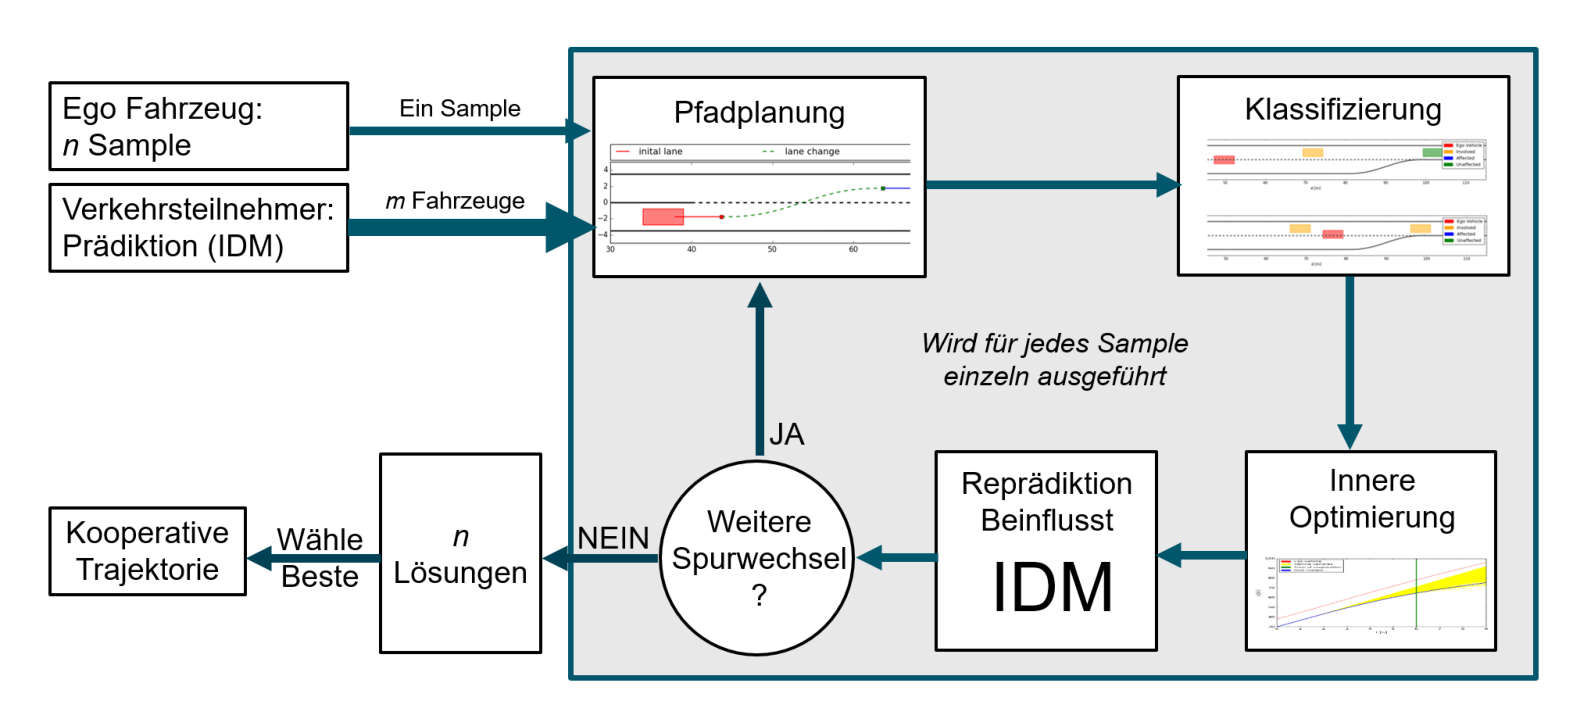
\includegraphics[width = 0.8 \textwidth ]{Ansatz.pdf}
    \caption[Planungsansatz]{Gesamt\"uberblick des Planungsansatzes. \textit{n} steht f\"ur die Anzahl der erzeugten Sample.}
    \label{fig:Ansatz}
 \end{figure}

In Abbildung~\ref{fig:Ansatz} ist ein Gesamt\"uberblick des Ansatzes visualisiert.
Auf wichtige Teilaspekte des Ansatzes wird in den nun folgenden Abschnitten genauer eingegangen.

\FloatBarrier


\subsection{Darstellung in Frenet Koordinaten}
\label{sec:FrenetBesch}
In Kapitel~\ref{sec:Frenet} wurde das Frenet"=Koordinatensystem vorgestellt und seine Verwendung in der Trajektorienplanung dieser Arbeit motiviert.
Eine Beschreibung in Frenet"=Koordinaten entspricht der mathematischen Beschreibung des Stra{\ss}enkoordinatensystems \cite{Rathgeber2016}.
Dabei wird eine Referenzkurve ausgew\"ahlt und die Planung findet dann entlang dieser Referenzkurve statt.
Die Fahrzeugposition wird nun durch die Bogenl\"ange \gls{symb:s_r} entlang der Referenzkurve und den Abstand \gls{symb:d_r} zur Referenzkurve beschrieben.

Es werden mehrere Vorteile genannt die sich durch die Verwendung der Frenet"=Koordinaten ergeben.
Unter anderem wird beschrieben, dass sich durch die Planung in Frenet"=Koordinaten auf einer gekr\"ummten Fahrbahn ein Fahrstreifenwechsel ergibt, der im Vergleich zu einer Planung in Weltkoordinaten mehr einem menschlichen Verhalten entspricht.
Dieser Effekt wird von Werling \cite{Werling2011} beschrieben und soll an dieser Stelle noch einmal genauer erl\"autert werden.

Im realen Verkehr ist h\"aufig ein Fahrstreifenwechsel zu beobachten, der auf gekr\"ummter Fahrbahn im Sinne von Komfort und Effizienz nicht dem Optimum entspricht.
So wird h\"aufig ein in Abbildung~\ref{fig:BeobaSpurwe} dargestellter Fahrstreifenwechsel beobachtet, obwohl der in Abbildung~\ref{fig:OptimalSpurwe} dargestellte Fahrstreifenwechsel aus Komfort- und Effizienzgr\"unden zu bevorzugen w\"are.
Grund daf\"ur ist, dass sich menschliche Fahrer bei der Planung des Fahrstreifenwechsel an den Fahrbahnmarkierungen orientieren.
Diese Planungsstrategie ist in Abbildung~\ref{fig:Planugsstrat} dargestellt.
Eine solche Planungsstrategie erleichtert die Bewegungspr\"adiktion f\"ur die umgebenden Fahrzeuge, da eine Realtivbewegung zur Stra{\ss}e fr\"uher als Absolutbewegung \"uber dem Untergrund wahrgenommen werden kann.
Ein Fahrstreifenwechsel wie in Abbildung~\ref{fig:OptimalSpurwe} dargestellt ist somit f\"ur andere Fahrer schwerer einzusch\"atzen und k\"onnte in dichtem Verkehr zu einer gef\"ahrlichen Situation f\"uhren. 
Deshalb ist auch f\"ur automatisierte Fahrzeuge die in Abbildung~\ref{fig:Planugsstrat} dargestellte Planungstrategie zu bevorzugen.
Eine solche Planungsstrategie ergibt sich, wenn in einer entkr\"ummenten Fahrzeugumgebung geplant wird.
Wie im Kapitel~\ref{sec:Frenet} beschrieben entspricht das einer Planung im Frenet"=Koordinatensystem.
Dies macht deutlich, dass der Pfad des Fahrzeuges in Frenet"=Koordinaten beschrieben werden sollte. \cite{Werling2011}


\begin{figure}[!htbp]
    \centering
    \subfigure[Kostenoptimaler Fahrstreifenwechsel]{
        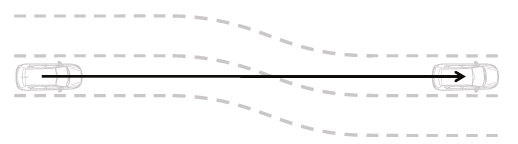
\includegraphics[width = 0.7 \textwidth]{Optimal.png}
        \label{fig:OptimalSpurwe}
    }
    \subfigure[Oft beobachter Fahrstreifenwechsel]{
        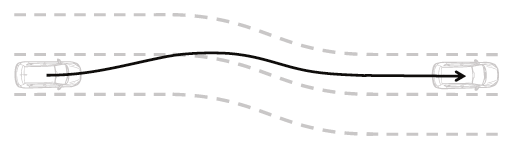
\includegraphics[width = 0.7  \textwidth]{Beobachtet.png}
        \label{fig:BeobaSpurwe}
    }
    \subfigure[Planugsstrategie von oft beobachteten Fahrstreifenwechseln]{
        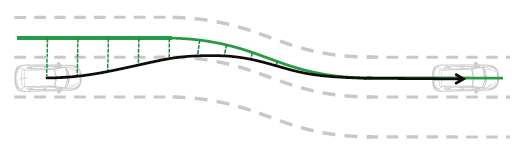
\includegraphics[width = 0.7  \textwidth]{Planungstrategie.png}
        \label{fig:Planugsstrat}
    }
    \caption[Fahrstreifenwechsel in Frenet"=Koordinaten]{Vergleich von unterschiedlichen Fahrstreifenwechselarten. \cite{Werling2011}}
    \label{fig:SimSzen}
\end{figure}


Wie wir in Kapitel~\ref{sec:Pfadplanung} sehen werden, ergibt sich der Pfad f\"ur einen einzelnen Fahrstreifenwechsel immer aus dem Pfad des aktuellen Fahrstreifens, dem Pfad des Zielfahrstreifens und einem verbindenden Zwischenst\"uck.
Zur Beschreibung in Frenet"=Koordinaten muss zus\"atzlich noch eine Referenzkurve gew\"ahlt werden.
Diese sollte m\"oglichst nahe an dem aktuellen Fahrstreifen und dem Zielfahrstreifen sein und au{\ss}erdem einen \"ahnlichen Verlauf haben, da so der Diskretisierungsfehler minimal gehalten werden kann.
Aus diesem Grund wird als Referenzkurve die Fahrbahnmakierung verwendet, die den aktuellen Fahrstreifen vom Zielfahrstreifen trennt.
Bei einem Fahrstreifenwechsel auf den linken Fahrstreifen w\"are dies zum Beispiel die rechte Fahrbahnmarkierung des Zielfahrstreifens.
Da ein doppelter Fahrstreifenwechsel innerhalb von einem Planungsschritt ausgeschlossen wird, sind dies die einzigen Verl\"aufe die zur Fahrstreifenwechselplanung notwendig sind.

Mit einem doppelten Fahrstreifenwechsel sind hierbei zwei Fahrstreifenwechsel in die gleiche Richtung gemeint.
Ein Fahrstreifenwechsel auf den Zielfahrstreifen und wieder zur\"uck auf den Ausgangsfahrstreifen wird dadurch nicht ausgeschlossen.
Dies ist f\"ur die Planung eines Fahrstreifenwechsels mit entgegenkommenden Verkehr wichtig.
Zwei direkt aufeinander folgende Fahrstreifenwechsel k\"onnen in dichtem Verkehr nur selten ausgef\"uhrt werden.
Ein solches Fahrverhalten birgt au{\ss}erdem ein erh\"ohtes Gefahren- und Unfallpotenzial.
Um einen doppelten Fahrstreifenwechsel sicher ausf\"uhren zu k\"onnen muss der Fahrer die Situation auf gleich mehreren Fahrstreifen \"uberblicken.
Zudem ist ein solches Fahrverhalten f\"ur andere Fahrer schwerer einzusch\"atzen.
Deshalb ist es zu bevorzugen zun\"achst einmal einen Fahrstreifenwechsel auszuf\"uhren und sich in den Verkehr des neuen Fahrstreifens einzugliedern.
Ist der Eingliederungsvorgang abgeschlossen kann der n\"achste Fahrstreifenwechsel geplant werden.
Ein solches Verhalten kann durch eine Planung, die zwar einen doppelten Fahrstreifenwechsel ausschlie{\ss}t aber in kurzen Zeitintervallen wiederholt wird, abgebildet werden.
Da eine kontinuierliche Neuplanung ohnehin unabdingbar ist, kann ein doppelter Fahrstreifenwechsel ohne gro{\ss}e Einschr\"ankungen ausgeschlossen werden.

Ist ein Fahrstreifenwechsel durchzuf\"uhren, der aufgrund des Ergebnisses der Routenplanung notwendig ist, sind au{\ss}er den Verl\"aufen der Referenzkurve und der Fahrstreifen noch weitere Informationen notwendig.
So muss bekannt sein bis wann und gegebenfalls auch ab wann ein Fahrstreifenwechsel durchgef\"uhrt werden kann.
Da ein kartenbasierter Ansatz angenommen wird, kann davon ausgegangen werden, dass sowohl diese Informationen als auch die Verl\"aufe der Fahrstreifen und der Referenzkurve gegeben sind.
Gegebenfalls muss noch eine Transformation von Welt- in Frenet"=Koordinaten stattfinden.

Wie in Kapitel~\ref{sec:Frenet} beschrieben erfolgt sowohl die Beschreibung der Fahrzeugeigenbewegung als auch die Beschreibung aller Kraftfahrzeuge in der Umgebung des Ego"=Fahrzeuges in Frenet"=Koordinaten.
Dazu wird die Bewegung der Fahrzeuge auf dem gegeben Pfad entlang der Referenzkurve berechnet.
Die Bewegung entlang der Referenzkurve ergibt sich aus dem Bewegungsanteil in Richtung der Referenzkurve w\"ahrende eines Zeitschrittes.
Bei gekr\"ummter Referenzkurve sollte die Kr\"ummung ebenfalls ber\"ucksichtig werden.
Damit ergibt sich die in Werling \cite{Werling2011} beschriebene Formel zur Berechnung der zur\"uckgelegten Wegstrecke entlang der Referenzkruve:

\begin{equation}
   \dot{s}_r = v \frac{\cos(\theta - \theta_\mathrm{ref})}{1 - d_r \kappa_\mathrm{ref}(s_r)}
\end{equation}

Dabei beschreiben \gls{symb:theta} und \gls{symb:theta_ref}die Richtung der Trajektorie und der Referenzkurve in Weltkoordinaten und \gls{symb:kappa_ref} die Kr\"ummung der Referenzkurve.
Das verwendete Frenet"=Koordinatensystem ist in Abbildung~\ref{fig:Frenet} dargestellt.

\begin{figure}[!htbp]
    \centering
    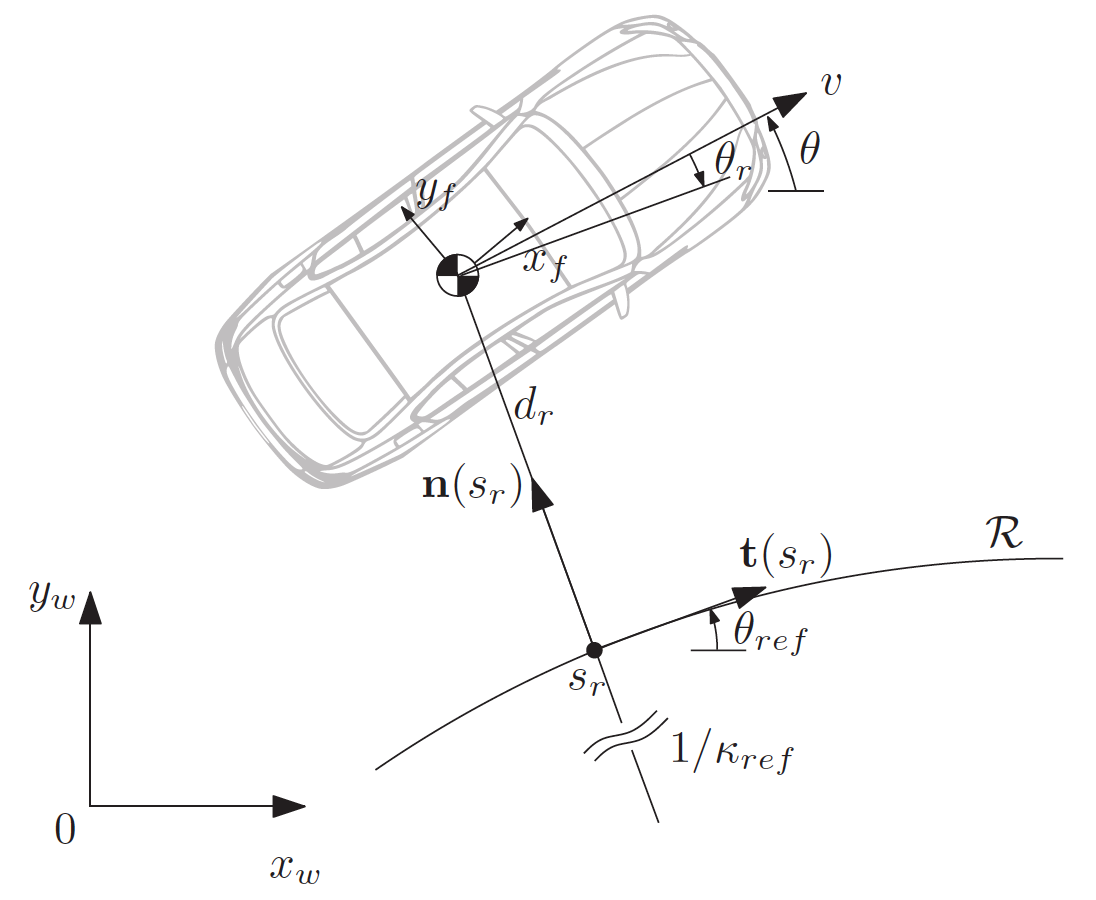
\includegraphics[width = 0.5 \textwidth ]{Frenet.png}
    \caption[Frenet"=Koordinatensystem]{Verwendetes Frenet"=Koordinatensystem \cite{Rathgeber2016}}
    \label{fig:Frenet}
\end{figure}


\FloatBarrier


\subsection{Kostenfunktional}
\label{sec:LCKostfunc}
In Kapitel~\ref{sec:Kostfunc} wird auf das Kostenfunktional des Basisalgorithmus eingegangen.
Dieses ber\"ucksichtigt die Kosten aller relevanten Fahrzeuge f\"ur den kompletten Planungshorizont.
Damit wird ein kooperatives Verhalten aller Verkehrsteilnehmer angenommen.
Es soll nun eine Situation betrachtet werden, in der sich hinter einem Fahrzeug auf dem selben Fahrstreifen ein anderes Fahrzeug befindet das eine h\"ohere Wunschgeschwindigkeit hat.
Durch das Abweichen von dieser Wunschgeschwindigkeit entstehen f\"ur das hintere Fahrzeug Kosten.
Durch das Gesamtkostenfunktional w\"urden sich diese Kosten auch auf das Verhalten des vorausfahrenden Fahrzeuges auswirken und dieses w\"urde wom\"oglich seine Geschwindigkeit erh\"ohen.
Ein solches Verhalten ist zu vermeiden, denn es w\"urde bedeuten, dass auf dr\"angelnde Fahrzeuge reagiert wird.
Dieses Szenario zeigt, dass es f\"ur die Trajektorieplanungen des Ego"=Fahrzeuges nicht sinnvoll ist alle Fahrzeuge im Kostenfunktional zu ber\"ucksichtigen.
Dies trifft besonders dann zu, wenn sich viele andere Fahrzeuge in der Umgebung des Ego"=Fahrzeuges befinden.
Es wird deshalb ein Kostenfunktional eingef\"uhrt, dass nur die Kosten von kooperierenden Fahrzeugen ber\"ucksichtigt und dies auch nur \"uber den Zeitraum in dem die Fahrzeuge ein kooperatives Verhalten zeigen.

Zur Beschreibung des Kostenfunktionals sollen nun folgende Zeitpunkte eingef\"uhrt werden:
\begin{itemize}
\item \gls{symb:t_lc} : Zeitpunkt an dem das Fahrzeug das einen Fahrstreifenwechsel beabsichtigt die Fahrbahnmakierung \"uberquert.
\item \gls{symb:t_coop,start}: Die Intension des Fahrstreifenwechsel wurde erkannt und die involvierten Fahrzeuge fangen an ihre Geschwindigkeit anzupassen.
\item \gls{symb:t_coop,end}: Der Fahrstreifenwechsel ist beendet. Die Fahrzeuge gehen in Folgefahrt bzw. freie Fahrt \"uber.
\end{itemize}

Zur Vereinfachung wird angenommen, dass \gls{symb:t_lc} der erste diskretisierte Zeitschritt ist, an dem sich das Ego"=Fahrzeuge teilweise auf dem Zielfahrstreifen befindet.
Der Zeitpunkt \gls{symb:t_coop,start} ist zeitlich vor \gls{symb:t_lc}.
Um diesen Zeitpunkt zu ermitteln muss in Betracht gezogen werden, wann es den umgebenden Fahrzeugen m\"oglich ist die Intension eines Fahrstreifenwechseles zu erkennen.
Befindet sich das Ego"=Fahrzeug auf einer Beschleunigungsspur ist davon auszugehen, dass die Intension von Anfang an bekannt ist.
Ansonsten kann mit guter N\"aherung davon ausgegangen werden, dass die Intension erkannt wird sobald der Fahrrichtungsanzeiger (Blinker) aktiviert wurde.
F\"ur \gls{symb:t_coop,end} wird davon ausgegangen, dass die Kooperation abgeschlossen ist, sobald der Fahrstreifenwechsel vollst\"andig durchgef\"uhrt wurde.
Das Ego"=Fahrzeug geht zur Folgefahrt zum vorderen Fahrzeug auf dem Zielfahrstreifen \"uber, das hintere zur Folgefahrt in Bezug auf das Ego"=Fahrzeug.
Damit kann die Kooperation auf den Zeitraum von \gls{symb:t_coop,start} bis  \gls{symb:t_coop,end} beschr\"ankt werden.
Dieser Zeitraum soll im weiteren als kooperativer Zeitraum bezeichnet werden.

In dem Kostenfunktional sollen nun die Kosten des Ego"=Fahrzeuges \"uber den kompletten Planungshorizont und die Kosten der kooperativen Fahrzeuge im Zeitraum von \gls{symb:t_coop,start} bis \gls{symb:t_coop,end} ber\"ucksichtigt werden.
Das Kostenfunktional kann also wie folgt aufgestellt werden

\begin{equation}
	G_\mathrm{total,lc} = G_\mathrm{ego} + \sum_{i = 1}^m G_i^{t,coop}
\end{equation}

\gls{symb:G_ego} beschriebt die Kosten des Ego"=Fahrzeuges \"uber den kompletten Planungshorizont. 
Mit \( m \) wird die Anzahl an kooperativen Fahrzeugen angegeben.
\gls{symb:G_coop} sind die Kosten der kooperativen Fahrzeuge w\"ahrend des kooperativen Zeitraumes.

Die Kosten der einzelnen Fahrzeug k\"onnen wie im Basisalgorithmus beschrieben, in die Kosten die nur die eigene Trajektorie betreffen und in Kosten die in Interaktion mit anderen Fahrzeugen entstehen eingeteilt werden.
Die Kosten die nur die eigene Trajektorie betreffen sollen im weiteren als dynamische Kosten bezeichnet werden.
Kosten die in Interaktion mit anderen Fahrzeugen auftreten werden als interaktive Kosten bezeichnet werden.
In den folgenden Abschnitten soll nun auf die einzelnen verwendeten Kostenterme eingegangen werden.

\minisec{Dynamische Kostenterme}
Bei dem in dieser Arbeit verwendeten Kostenfunktional setzt sich der Anteil der Terme, die nur die eigene Trajektorie betreffen, aus den Termen \gls{symb:G_v} und \gls{symb:G_a} zusammen.
\gls{symb:G_v} beschreibt die Kosten die durch das Abweichen von einer optimalen Geschwindigkeit entstehen.
\gls{symb:G_a} diejenigen Kosten die durch das Auftreten von tangentialen Beschleunigungen entstehen.
Auf die Ber\"ucksichtigung von R\"ucken sowie lateralen Beschleunigungen wird verzichtet.
Der Ruck ist die Ableitung der Beschleunigung.
Die zuf\"allig ermittelten R\"ucke werden beim Generieren der Geschwindigkeitsprofile so begrenzt, dass ausschlie{\ss}lich R\"ucke entstehen, die als angenehm wahrgenommen werden.
Auch laterale Beschleunigungen nehmen bei Einhaltung der H\"ochstgeschwindigkeit in der Regel keine allzu gro{\ss}en Werte an, da der Fahrbahnverlauf entsprechend ausgelegt wurde.
An Streckenabschnitten bei denen dennoch hohe laterale Beschleunigungen entstehen, kann dem durch Anpassen der Optimalgeschwindigkeit des Fahrzeuges entgegengewirkt werden.
Auch beim Fahrstreifenwechsel des Ego"=Fahrzeuges ist nicht von hohen lateralen Beschleunigungen auszugehen, da er, wie wir in Kapitel~\ref{sec:Pfadplanung} sehen werden, auf die Geschwindigkeit des Fahrzeuges angepasst ist.

F\"ur das Ego"=Fahrzeug wird als Optimalgeschwindigkeit standartm\"a{\ss}ig die erlaubte H\"ochstgeschwindigkeit angenommen.
Dieser Wert kann aufgrund des Streckenverlaufs angepasst werden.
F\"ur alle anderen Fahrzeuge wird die bis dahin h\"ochste gemessene Geschwindigkeit als optimale Geschwindigkeit angenommen, solange es zu keiner \"Anderung der erlaubten Maximalgeschwindigkeit kommt.
Bei den in \cite{Naumann2017towards} simulierten Szenarien wurde f\"ur die negative Abweichung von der Maximalgeschwindigkeit kein diskomfortabler Bereich eingef\"uhrt.
Dies ergibt Sinn, wenn betrachtet wird, dass beispielsweise in einem Stau die Kosten aufgrund der starken Abweichung zur Optimalgeschwindigkeit stark ansteigen.
Dies k\"onnte zu \"uberm\"a{\ss}ig hohen Beschleunigungen beim Anfahren oder h\"aufigen Fahrstreifenwechseln f\"uhren, da das Fahrzeug bestrebt ist seine Geschwindigkeit m\"oglichst schnell der Optimalgeschwindigkeit anzupassen.
Allerdings kann auch ein starkes Abweichen von der erlaubten Maximalgeschwindigkeit bis hin zum Stehenbleiben zu gef\"ahrlichen Situationen f\"uhren und sollte deshalb vermieden werden.
Bei nur schwach ansteigenden Kosten beim Abweichen von der Wunschgeschwindigkeit wird dies m\"oglicherweise nicht hinreichend abgebildet.
Aus diesem Grund wird vorgeschlagen, eine Diskomfortgrenze einzuf\"uhren, die allerdings von der durchschnittlichen Geschwindigkeit aller Fahrzeuge in der Umgebung abh\"angt.
Auf diese Weise k\"onnen beide Aspekte ber\"ucksichtig werden.

\minisec{Interaktive Kostenterme}
Der Kostenanteil der durch Interaktion mit anderen Fahrzeugen entsteht setzt sich aus den Kostentermen \gls{symb:G_sd}, \gls{symb:G_lc} und \gls{symb:G_lcend} zusammen.
Durch \gls{symb:G_sd} wird das Unterschreiten von Sicherheitsabst\"anden bestraft.
Mit \gls{symb:G_lc} das Schneiden eines Fahrzeuges auf dem Zielfahrstreifen.
\gls{symb:G_lcend} bewertet, wie stark ein kooperierendes Fahrzeug am Ende des kooperativen Planungshorizonts von seiner Wunschgeschwindigkeit abweicht.

Als Sicherheitsabstand muss immer so viel Abstand zu dem vorausfahrenden Fahrzeug gehalten werden, dass bei einer Vollbremsung des vorausfahrenden Fahrzeuges das eigene Fahrzeug in der Lage ist hinter dem vorausfahrenden Fahrzeug zum Stehen zu kommen.
Dabei muss auch eine Reaktionszeit ber\"ucksichtigt werden.
Diese beschreibt die Zeit die gebraucht wird um auf die Vollbremsung des vorausfahrenden Fahrzeuges zu reagieren.
Bei einem Menschen wird eine Reaktionszeit von circa einer Sekunde angenommen.
Diesen Sicherheitsabstand durchgehend zu berechnen ist f\"ur einen Menschen eine unl\"osbare Aufgabe.
Es hat sich deshalb die Faustformel etabliert, dass der Sicherheitsabstand den halben Wert der Tachoanzeige in Metern ergeben muss.
Bei einer gefahrenen Geschwindigkeit von 80 km/h muss demnach ein Abstand von 40 Metern eingehalten werden.
Zur Orientierung k\"onnen die Leitpfosten am Fahrbahnrand verwendet werden.
Diese stehen in Deutschland etwa 50 Meter weit auseinander.
Ist dieser Abstand eingehalten, ist in der Regel auch der notwendige Sicherheitsabstand eingehalten.
Der nach dieser Formel berechnete Abstand entspricht einem Zeitabstand (englisch: time headway) \gls{symb:t_abs} zum vorausfahrenden Fahrzeug.
Auch in dieser Arbeit wird der nach der Faustformel berechnete Zeitabstand \gls{symb:t_abs} als Grundlage zu Berechnung des Kostenterms \gls{symb:G_sd} verwendet.
Der Zeitabstand kann jedoch auch durch einen anderen Wert ersetzt werden, wenn beispielsweise in anderen L\"andern durch eine Regelung andere Zeitabst\"ande gefordert sind.

Im realen Verkehr ist oft ein leichtes Schneiden der Fahrzeuge auf dem Zielfahrstreifen zu beobachten.
Das hei{\ss}t, dass die L\"ucke auf dem Zielfahrstreifen bei Einleitung des Fahrstreifenwechsels noch nicht so gro{\ss} ist, dass sowohl zum vorausfahrenden Fahrzeug als auch zum folgenden Fahrzeug der geforderte Zeitabstand eingehalten wird.
Diese L\"ucke vergr\"o{\ss}ert sich w\"ahrend des Fahrstreifenwechsels noch und sollte sp\"atestens bei Beendigung des Fahrstreifenwechsel so gro{\ss} sein, dass die entsprechenden Abst\"ande eingehalten werden.
Dieses Verhalten ist akzeptabel, da der Fahrstreifenwechsel bis zu einem gewissen Zeitpunkt noch abgebrochen werden kann.
Au{\ss}erdem werden in Deutschland laut Rechtssprechnung des Bundesgerichtshofes ganz vorr\"ubergehende Unterschreitungen der Sicherheitsabst\"ande nicht geahndet \gls{judica}.
Dieses Fahrverhalten soll auch dem Ego"=Fahrzeug erlaubt sein.
Es vereinfacht bei dichtem Verkehr in vielen F\"allen das Auffahren auf den Zielfahrstreifen.
Au{\ss}erdem ist der Abstand der durch die Faustformel gegeben ist in der Regel gr\"o{\ss}er als der tats\"achlich notwendige Sicherheitsabstand.
Um dieses Verhalten zu realisieren wird um den vorderen Bereich der Fahrzeuge ein Sicherheitsbereich in Form einer halben Ellipse eingef\"uhrt.
Die Breite der Ellipse h\"angt von der Fahrstreifenbreite ab.
Die L\"ange der Ellipse ergibt sich aus dem geforderten Zeitabstand \gls{symb:t_abs}.
Der Sicherheitsbereich ist in Abbildung~\ref{fig:NormSD} visualisiert.
Eine solche Form als Sicherheitsbereich sorgt daf\"ur, dass ein Einscheren direkt vor dem Folgefahrzeug vermieden wird. 
Das Schneiden findet erst statt wenn bereits ein Abstand erreicht ist, der vergleichsweise nahe an dem geforderten Sicherheitsabstand ist.
Schwarting et al. \cite{Schwarting2014} verwenden einen \"ahnlichen Ansatz.
Hier wird um die Fahrzeuge eine ellipsenf\"ormige Sicherheitszone erzeugt um Konflikte mit anderen Fahrzeugen zu ermitteln.

\begin{figure}[!htbp]
    \centering
    \subfigure[Sicherheitsabstand wird eingehalten (\( d_\mathrm{normal} = 1,09 \)). ]{
        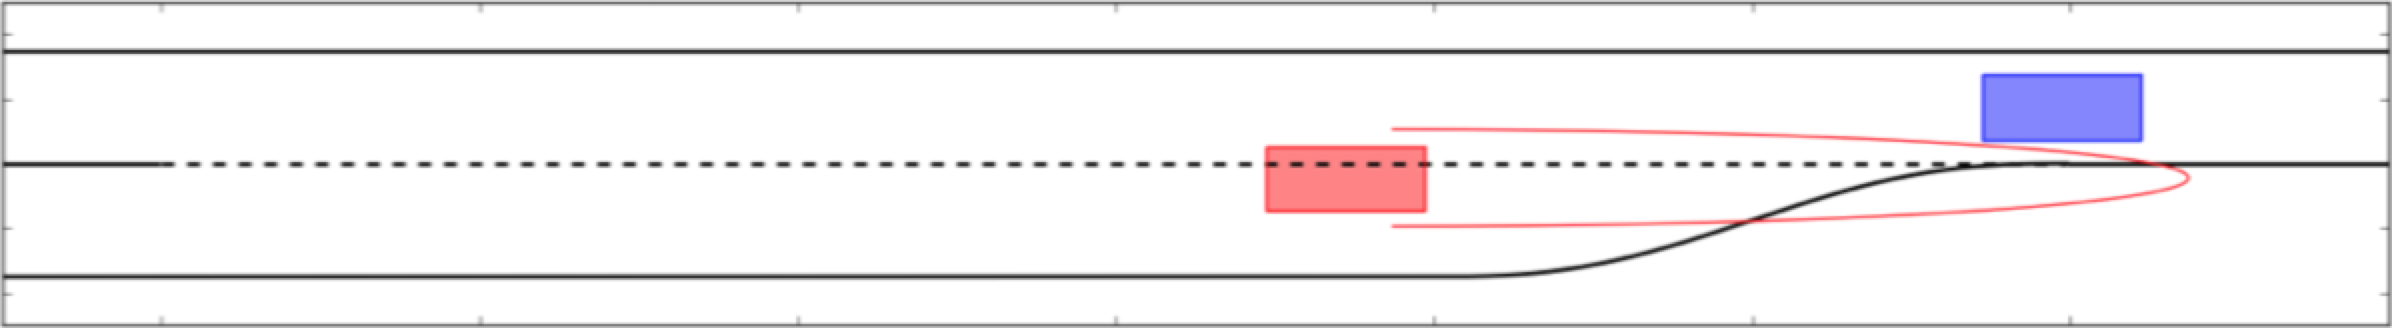
\includegraphics[width =  \textwidth]{Einhalten.png}
    }
    \subfigure[Sicherheitsabstand wird unterschritten (\( d_\mathrm{normal} = 0,85 \)).]{
        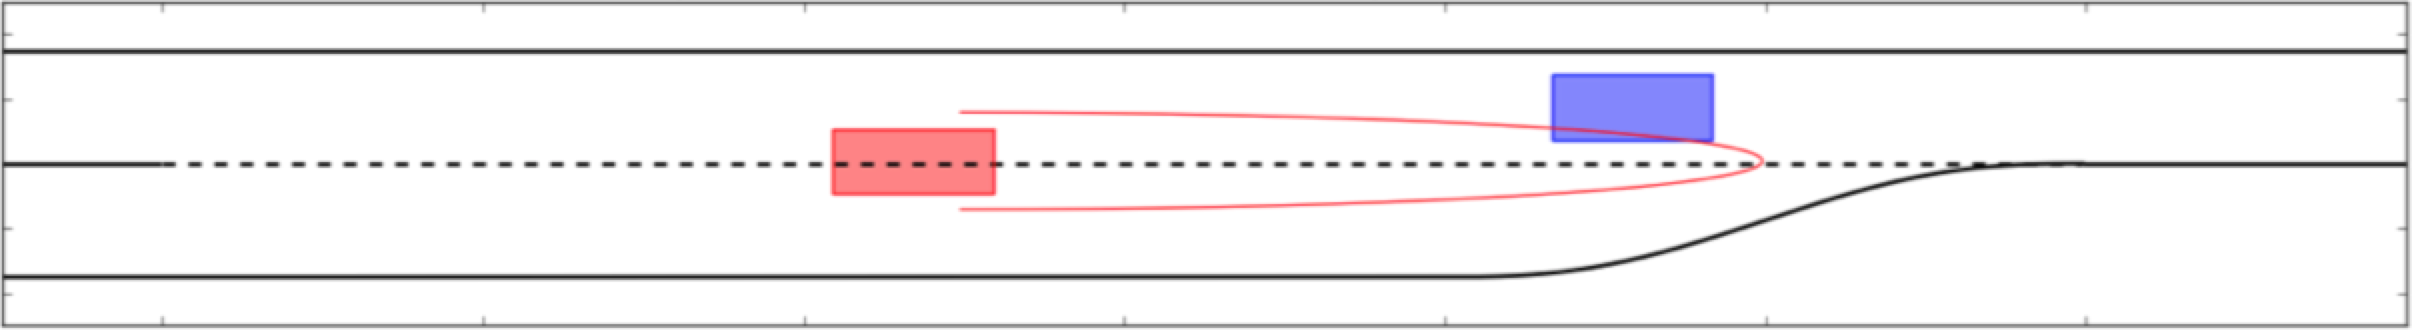
\includegraphics[width =  \textwidth]{Unterschreiten.png}
    }
    \caption[Normalisierter Sicherheitsabstand]{Normalisierter Sicherheitsabstand}
    \label{fig:NormSD}
\end{figure}



Um nun den Kostenterm \gls{symb:G_sd} zu berechnen wird ein normalisierter Sicherheitsabstand \gls{symb:d_normal} eingef\"uhrt.
Dieser hat den Wert Eins wenn sich ein anderes Fahrzeuge gerade am Rand des Sicherheitsbereiches befindet und den Wert Null wenn sich die beiden Fahrzeug gerade ber\"uhren.
Zwischen diesen beiden Werten wird linear interpoliert.
Durch den Kostenterm \gls{symb:G_sd} werden nun alle Abst\"ande die zu einem normalisierten Sicherheitsabstand f\"uhren der einen festgelegten Grenzwert unterschreitet mit entsprechenden Kosten bewertet.
Da ein Unterschreiten des Sicherheitsabstandes besonders sicherheitskritisch ist und von Menschen schnell als unangenehm empfunden wird, sollten die Kosten f\"ur das Unterschreiten des Sicherheitsabstandes vergleichsweise stark ansteigen.
Deshalb wird die Grenze zum diskomfortablen Bereich relativ nahe am Optimum gew\"ahlt.

Bei einem Fahrstreifenwechsel sollten die Fahrzeuge auf dem Zielfahrstreifen nicht zu einem sicherheitskritischem Bremsman\"over gezwungen werden \cite{Treiber2010}.
Im Idealfall findet der Fahrstreifenwechsel so statt, dass keine Verz\"ogerung notwendig ist.
Es wird deshalb der Kostenterm \gls{symb:G_lc} eingef\"uhrt. 
Damit werden Verz\"ogerungen bewertet zu denen die Fahrzeuge auf dem Zielfahrstreifen gezwungen w\"aren, wenn sie bis zum Ende des Fahrstreifenwechsels den geforderten Zeitabstand  \gls{symb:t_abs} einhalten wollen.
Dabei wird davon ausgegangen, dass die Verz\"ogerung bei \gls{symb:t_lc} eingeleitet wird und der Abstand bei \gls{symb:t_coop,end} genau eingehalten wird.
Am Ende des Fahrstreifenwechsels soll nun also ein Abstand \gls{symb:d_sd} eingehalten werden, der mit dem gew\"unschten Zeitabstand \gls{symb:t_abs} wie folgt berechnet wird:

\begin{equation}
	d_\mathrm{sd} =  T_\mathrm{abs}  v_\mathrm{t,lc}^{follow}.
\end{equation}

Der Wert \(v_\mathrm{t,lc}^{follow}\) beschreibt die Geschwindigkeit des Folgefahrzeuges auf dem Zielfahrstreifen zum Zeitpunkt \gls{symb:t_lc}.
Der Abstand \( d_\mathrm{t,end,coop}\) der beiden Fahrzeuge am Ende des Verz\"ogerungsvorgangs kann wie folgt berechnet werden:

\begin{equation}
	d_\mathrm{t,end,coop} = d_\mathrm{t,lc} + v_\mathrm{t,lc}^{change} \Delta t- \left( v_\mathrm{t,lc}^{follow} \Delta t+ 0,5 * b_\mathrm{nece} \Delta t^2 \right)
\end{equation}

Dabei ist \gls{symb:d_tlc} der Abstand der beiden Fahrzeuge zum Zeitpunkt \gls{symb:t_lc}, \(v_\mathrm{t,lc}^{change}\) die Geschwindigkeit des fahrstreifenwechselnden Fahrzeuges zum Zeitpunkt \gls{symb:t_lc} und \gls{symb:b_nece} die gesuchte notwendige Verz\"ogerung.
Der Wert \(\Delta t\)  ergibt sich zu \gls{symb:t_coop,end} - \gls{symb:t_lc}.
Durch Gleichsetzten von \gls{symb:d_sd} und \(d_\mathrm{t,end,coop}\) und anschlie{\ss}endem ausfl\"osen nach \(b_\mathrm{nece}\) ergibt sich die folgende Formel:

\begin{equation}
	b_\mathrm{nece} = \frac{d_\mathrm{t,lc} + \left( v_\mathrm{t,lc}^{change} - v_\mathrm{t,lc}^{follow} \right) \Delta t -    T_\mathrm{abs} v_\mathrm{t,lc}^{follow}}{T_\mathrm{abs}  \Delta t + 0,5 * \Delta t^2}
\end{equation}
Durch den Kostenterm \gls{symb:G_lc} werden nur negative Werte von \gls{symb:b_nece} mit Kosten bewertet.


Dadurch dass die Kosten der kooperativen Fahrzeuge nur bis \gls{symb:t_coop,end} ber\"ucksichtigt werden und die Kosten des Ego"=Fahrzeuges dar\"uber hinaus, wird das Ego"=Fahrzeug in der Optimierung bevorzugt.
Bei der gleichen Trajektorie des Ego"=Fahrzeuges und eines kooperativen Fahrzeuges verursacht die Trajeketorie des Ego"=Fahrzeuges bei gleichem Kostenfunktional h\"ohere Kosten, da sie auch nach \gls{symb:t_coop,end} Kosten verursacht.
Zur Minimierung der Kosten wird deshalb ein Trajektorieset angestrebt bei dem die Geschwindigkeit des Ego"=Fahrzeuges m\"oglichst nahe an dessen Optimalgeschwindigkeit ist.
Die Geschwindigkeitsabweichnung des kooperativen Fahrzeuges f\"allt weniger ins Gewicht.
Um dies zu vermeiden wird der Kostenterm \gls{symb:G_lcend} eingef\"uhrt.
Durch ihn wird der Zustand der kooperierenden Fahrzeuge zum Zeitpunkt \gls{symb:t_coop,end} bewertet.
Dadurch k\"onnen auch Kosten \"uber \gls{symb:t_coop,end} hinaus abgebildet werden.

Zur Berechnung des Kostenterms wird eine Beschleunigung \gls{symb:a_lcend} aus dem komfortablen Bereich gew\"ahlt.
Anschlie{\ss}end wird berechnet welche Zeit \(t_\mathrm{accel}\) ben\"otigt wird um vom Zustand des kooperativen Fahrzeuges zum Zeitpunkt \gls{symb:t_coop,end}  auf die gew\"unschte Optimalgeschwindigkeit zu beschleunigen.
Dabei wird von einer konstanten Beschleunigung mit \gls{symb:a_lcend} ausgegangen.
Es wird au{\ss}erdem die mittlere Geschwindigkeit \( \bar{v}_\mathrm{lc,end} \) f\"ur den Beschleunigungsvorgang bestimmt.
Der Kostenterm \gls{symb:G_lcend} ergibt sich nun aus der Berechnung der dynamischen Kosten bei einer konstanten Beschleunigung \(a_\mathrm{lc,end} \) und einer als konstant angenommenen Geschwindigkeit  \( \bar{v}_\mathrm{lc,end} \) \"uber einen Zeitraum von \gls{symb:t_coop,end} bis \gls{symb:t_coop,end} +  \( t_\mathrm{accel}\).
Ist  \gls{symb:t_coop,end} +  \(t_\mathrm{accel}\) gr\"o{\ss}er als der Planungshorizont werden die dynamischen Kosten von \gls{symb:t_coop,end} bis zum Ende des Planungshorizonts berechnet.


\subsection{Fahrstreifenbasierte Pr\"adiktion}
\label{sec:IDMpred}
Die Bewegunspr\"adiktion anderer Fahrzeuge ist eine entscheidende Herausforderung f\"ur automatisierte Fahrzeuge.
Hier wird pr\"adiziert, wie sich eine Verkehrssituation in n\"achster Zukunft entwickeln wird.
Dabei werden die zuk\"unftigen Positionen und Zust\"ande der einzelnen Fahrzeuge vorherbestimmt \cite{Hermes2009}.
Dies ist notwendig um potentielle Risiken m\"oglichst fr\"uh zu erkennen.
Beruhend darauf kann dann eine Trajektorieplanung stattfinden.

Grundsteine von Bewegungspr\"adiktionen sind Bewegungsmodelle.
Durch sie wird bestimmt, wie sich die Fahrzeuge im aktuellen Szenario verhalten werden.
Lef\`{e}vre et al. \cite{Lefevre2014} teilen die Bewegungsmodelle in drei Gruppen steigender Komplexit\"at auf:

\begin{enumerate}
\item \textit{Physik"=basierte Bewegungsmodelle}: Die Bewegung der Fahrzeuge h\"angt ausschlie{\ss}lich von Gesetzten der Physik ab
\item \textit{Man\"overbasierte Bewegungsmodelle}: Die Bewegung h\"angt zus\"atzlich von Man\"overn ab, die der Fahrer plant durchzuf\"uhren
\item \textit{Interaktionsber\"ucksichtigende Bewegungsmodelle}: Die Wechselbeziehung von Man\"overn verschiedener Fahrzeuge wird ber\"ucksichtigt.
\end{enumerate}

Zu den einfachsten Bewegungsmodellen geh\"oren die Bewegungsmodelle der konstanten Geschwindigkeit und der konstanten Beschleunigung.
Sie werden den Physik"=basierten Bewegungsmodellen zugeordnet.
Physik"=basierte Bewegungsmodelle sind die am meisten benutzten Bewegungsmodelle zur Trajektorienp\"ardiktion \cite{Lefevre2014}.
Allerdings sind sie auf sehr kurze Pr\"adiktionshorizonte limitiert, da sie nicht auf Ver\"anderungen der direkten Fahrzeugumgebung, wie einem langsam fahrenden Fahrzeug, reagieren k\"onnen.
Werden andere Aspekte wie Unsicherheiten bei der Sch\"atzung der aktuellen Fahrzeugzust\"ande und Interaktionen zwischen Fahrzeugen ber\"ucksichtigt nimmt die Komplexit\"at stark zu.

Wird jedoch angenommen, dass keines der Fahrzeuge w\"ahrend des Planungshorizonts seinen Fahrstreifen wechselt, vereinfacht sich die Situation erheblich.
Das Bewegungsmodell h\"angt nun ma{\ss}geblich von der eigenen Wunschgeschwindigkeit und dem vorausfahrenden Fahrzeug ab.
Damit kann auf g\"angige Einspur"=Fahrzeugfolgemodelle zur\"uckgegriffen werden.
Auch heutige Adaptive Cruise Control (ACC) Systeme beruhen auf Modellen dieser Art.
Der Schwerpunkt dieser Arbeit liegt nicht auf der Bewegungsp\"adiktion.
Deshalb soll die vereinfachende Annahme getroffen werden, dass alle anderen Fahrzeuge in der Umgebung des Ego"=Fahrzeuges ihren Fahrstreifen innerhalb des Planungshorizontes beibehalten.
Damit kann sowohl f\"ur die vom Ego"=Fahrzeug unabh\"angige Bewegunspr\"adiktion also auch f\"ur die Neupr\"adiktion nach dem Fahrstreifenwechsel ein Fahrzeugfolgemodel verwendet werden.
Die Pr\"adiktion findet f\"ur jeden Fahrstreifen einzeln statt.
Diese Annahme kann jedoch durch Verwendung eines anderen Pr\"adiktionsverfahren aufgelockert werden.
F\"ur das Einspur"=Fahrzeugfolgemodel wurde sich f\"ur das von Treiber et al. \cite{Treiber2000} vorgestellte \gls{idm} entschieden.
Dies wird im Folgenden vorgestellt.


\minisec{Intelligent Driver Model}
Das Intelligent Driver Model ist ein zeitkontinuierliches Einspur"=Fahrzeugmodell.
Es geh\"ort zu einem der bekanntesten und meist angewendeten Fahrzeugmodellen.
Es wird unter anderem in \cite{Schwarting2014} und \cite{Hubmann2018} verwendet um das Standartverhalten der Fahrzeuge abzubilden.
Laut Schwarting et al. \cite{Schwarting2014} ist damit eine realistische Simulation der Verkehrsszene innerhalb des Planungshorizonts m\"oglich.
Dies gilt nur unter der Annahme, dass keine Fahrstreifenwechsel stattfinden.
Das \gls{idm} weist einige Vorteile gegen\"uber anderen Einspur"=Fahrzeugfolgemodellen auf.
So werden realistische Beschleunigungen ermittelt, es werden keine Unf\"alle erzeugt und es ist auch bei nicht dichtem Verkehr anwendbar.
Die Fahrzeugdynamik wird, wie bei den meisten Fahrzeugfolgemodellen, durch eine Beschleunigungsfunktion beschrieben \cite{Treiber2000}.
Durch Integration der Beschleunigung kann dann die Geschwindigkeit und die Position des Fahrzeuges berechnet werden.
In Vergleich zu anderen Fahrzeugefolgemodellen werden viele Parameter ber\"ucksichtigt:

\begin{itemize}
\item \textit{Wunschgeschwindigkeit} \( v_{0} \): Die Geschwindigkeit, die das Fahrzeug ohne Verkehr fahren w\"urde
\item \textit{Minimalabstand} \(s_{0}\): Minimal gew\"unschter Abstand zum vorausfahrenden Fahrzeug
\item \textit{Gew\"unschte Zeitl\"ucke} \( T \): Gew\"unschter Zeitabstand zum vorausfahrenden Fahrzeug
\item \textit{Maximale Beschleunigung} \( a \): Maximale Beschleunigung des Fahrzeuges
\item \textit{Komfortable Verz\"ogerung} \( b \): Verz\"ogerung die beim Bremsen gerade noch als komfortabel angesehen wird. (Es wird ein positiver Wert eingesetzt)
\item \textit{Beschleunigungsexponent} \( \delta \): Beschreibt wie die Beschleunigung beim Ann\"ahern an die Zielgeschwindigkeit abklingt
\item \textit{Geschwindigkeitsunterschied} \( \Delta v_\alpha \): Aktueller Geschwindigkeitsunterschied zwischen den beiden Fahrzeugen
\item \textit{Abstand \( s_\alpha \)}: Aktueller Abstand zwischen den beiden Fahrzeugen, gemessen von der Sto{\ss}stange des Fahrzeuges bis zum Heck des vorausfahrenden Fahrzeuges.
\end{itemize}

Es ergibt sich folgende Formel:

\begin{equation}
   \dot{v}_\alpha = a \left( 1 - \left( \frac{v_\alpha}{v_0}^\delta \right) - \left( \frac{s^*(v_\alpha, \Delta v_\alpha)}{s_\alpha}\right)^2\right).
\end{equation}

Es wird sowohl die aktuelle Geschwindigkeit \( v_\alpha\) mit der Wunschgeschwindigkeit \( v_{0} \) verglichen als auch der aktuelle Abstand \( s_\alpha \) mit dem Wunschabstand \( s^*\).
Der Wunschabstand
\begin{equation}
   s^*(v_\alpha, \Delta v_\alpha) =  s_0 + max \left( 0, v_\alpha T + \frac{v_\alpha \Delta v_\alpha}{2 \sqrt{ab}}\right)\end{equation}
enth\"alt neben einem Gleichgewichtsanteil \(s_0 + v_\alpha T \) auch einen dynamischen Anteil gegeben durch \( (v_\alpha \Delta v_\alpha)/(2 \sqrt{ab}) \).

Die Beschleunigungsformel l\"asst sich in einen freie Fahrt Term

\begin{equation}
   \dot{v}_\alpha^{free} = a \left( 1 - \left( \frac{v_\alpha}{v_0} \right) ^\delta \right)
\end{equation}

und einen interaktiven Term 

\begin{equation}
   \dot{v}_\alpha^{int} = - a \left( \frac{s^*(v_\alpha, \Delta v_\alpha)}{s_\alpha} \right)^2
\end{equation}

einteilen.
Der Term \( \dot{v}_\alpha^{free} \) beschreibt das Verhalten des Fahrzeuges bei freier Fahrt.
Der Term \( \dot{v}_\alpha^{int} \) beschreibt das Verhalten des Fahrzeuges wenn es aufgrund des Verkehrs nicht mehr mit der Wunschgeschwindigkeit fahren kann.


\subsection{Pfadplanung}
\label{sec:Pfadplanung}
Ein Pfad f\"ur einen einzelnen Fahrstreifenwechsel kann in drei Teilabschnitte eingeteilt werden: dem Pfad des aktuellen Fahrstreifens, dem Pfad des Zielfahrstreifens und dem Fahrstreifenwechselpfad.
Die drei Teilabschnitte sind in Abbildung~\ref{fig:Pfad} dargestellt.
Soll eine Trajektorie mehr als einen Fahrstreifenwechsel beinhalten, kann der Pfad aus mehreren einzelnen Fahrstreifenwechseln zusammengesetzt werden.
Die Funktion \gls{symb:F_init} zur Beschreibung des Pfades des aktuellen Fahrstreifen und die Funktion \gls{symb:F_target} zur Beschreibung des Pfades des Zielfahrstreifen sollen als gegeben angenommen werden.
Der Verlauf dieser Pfade ist durch die Fahrbahnmakierungen weitestgehend vorgegeben und kann in einer Karte hinterlegt werden.
In den meisten F\"allen wird der Verlauf angen\"ahert durch einen Polygonzug beschrieben.
Um den Pfad f\"ur das komplette Fahrstreifenwechselman\"over vollst\"andig beschreiben zu k\"onnen m\"ussen noch die geometrischen Punkte \( P_\mathrm{lc}^\mathrm{start}\) und \( P_\mathrm{lc}^\mathrm{end}\) festgelegt werden.
Sie beschrieben an welchem Punkt der Fahrstreifenwechsel eingeleitet wird und an welchem Punkt der Fahrstreifenwechsel beendet ist.
Des Weiteren muss die geometrische Verbindung der Punkte festgelegt werden.

\begin{figure}[!htbp]
    \centering
    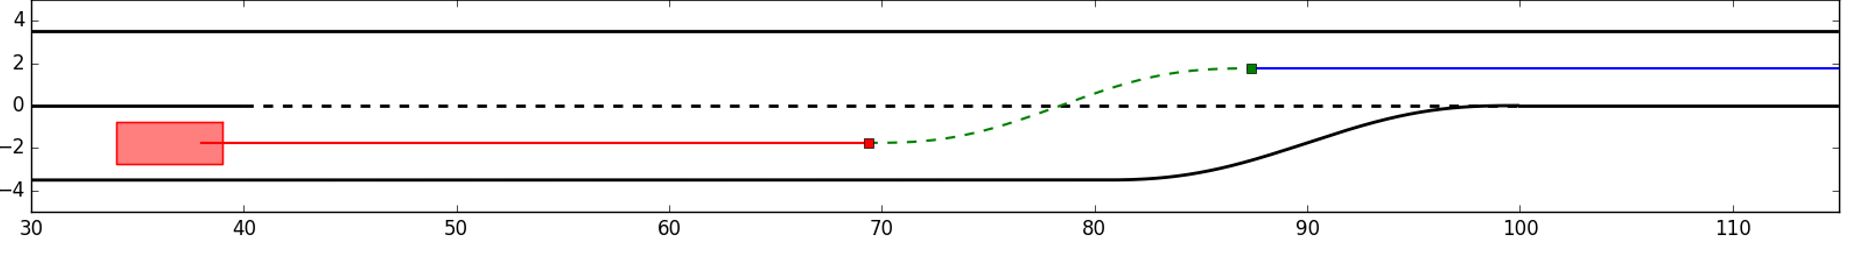
\includegraphics[width = 0.95 \textwidth ]{Pfad.png}
    \caption[Pfadplanung]{Pfad f\"ur einzelnen Fahrstreifenwechsel zusammengesetzt aus: Pfad des aktuellen Fahrstreifens (rot durchgezogen), Fahrstreifenwechselpfad (gr\"un gestrichelt), Pfad des Zielfahrstreifens (blau durchgezogen). Au{\ss}erdem dargestellt  \( P_\mathrm{lc}^\mathrm{start}\) (rot) und \( P_\mathrm{lc}^\mathrm{end}\) (blau)}
    \label{fig:Pfad}
\end{figure}


Wie in Kapitel~\ref{sec:FrenetBesch} erl\"autert, findet die Pfadplanung in Frenet"=Koordinaten statt.
Es ist au{\ss}erdem festgelegt, dass der Punkt \( P_\mathrm{lc}^\mathrm{start}\) auf dem Pfad des aktuellen Fahrstreifens liegt und das der Punkt \( P_\mathrm{lc}^\mathrm{end}\) auf dem Pfad des Zielfahrstreifens liegt.
Die Punkte sind demnach vollst\"andig beschrieben, wenn bekannt ist ab welcher Wegstrecke \gls{symb:s_cs} entlang der Referenzkurve der Fahrstreifenwechsel beginnt und ab welcher Westrecke \gls{symb:s_ce} der Fahrstreifenwechsel endet.
Die Funktion \gls{symb:F_lc}(s) zur Beschreibung des Gesamtpfades kann also wie folgt formuliert werden:

\begin{equation}
  F_\mathrm{lc}(s) = 
  \begin{cases} 
    F_\mathrm{init}                         & \quad , s \leq s_\mathrm{change}^\mathrm{start}\\ 
    F_\mathrm{change}                  & \quad , s_\mathrm{change}^\mathrm{start} < s \leq s_\mathrm{change}^\mathrm{end}\\ 
    F_\mathrm{target}                     & \quad , s > s_\mathrm{change}^\mathrm{end}.
  \end{cases} 
  \label{eqn:Kostenfunktion}
\end{equation}

Dabei ist \gls{symb:F_change} die Funktion des Fahrstreifenwechselpfades in Frenet"=Koordinaten.
Die noch zu ermittelnden Unbekannten sind der Start des Fahrstreifenwechsels \gls{symb:s_cs}, das Ende des Fahrstreifenwechsels \gls{symb:s_ce} und die Funktion \gls{symb:F_change}, die die beiden Punkte verbindet.
Die Pfadplanung soll aufgrund eines vorgegebenen Geschwindigkeitsprofiles generiert werden.

\minisec{Ermittlung des Fahrstreifenwechselsstartpunktes}
Um den Startpunkt des Fahrstreifenwechsels zu ermitteln ist es zun\"achst sinnvoll, noch einmal zu betrachten, aus welchen Gr\"unden Fahrstreifenwechsel durchgef\"uhrt werden.
Wie in Kapitel~\ref{sec:AuswahlBA} beschrieben, werden Fahrstreifenwechsel in notwendige und frei verf\"ugbare Fahrstreifenwechsel eingeteilt.
Fahrstreifenwechsel k\"onnen entweder notwendig sein, um einem vorgegebenen Pfad zu folgen oder weil der aktuelle Fahrstreifen endet.
Ein freiwilliger Fahrstreifenwechsel wird in der Regel durchgef\"uhrt um m\"oglichst mit der aktuellen Wunschgeschwindigkeit zu fahren.

Der einfachste Fall zur Bestimmung des Startpunktes des Fahrstreifenwechsels ergibt sich, wenn vorgegeben ist, dass sich am Ende des aktuellen Fahrstreifens nach dem Rei{\ss}verschlussverfahrens auf dem Zielfahrstreifen einzuordnen ist.
Der Bereich in dem der Fahrstreifenwechsel eingeleitet werden sollte ist somit stark eingeschr\"ankt.
Bei einer Beschleunigungsspur gilt das Rei{\ss}verschlussverfahren nicht.
Das gleiche gilt f\"ur Fahrstreifenwechsel die aufgrund der vorgegebenen Route durchgef\"uhrt werden m\"ussen.
Bei Fahrstreifenwechseln dieser Art ist deutlich schwerer festzulegen, wann ein Fahrstreifenwechsel eingeleitet werden soll.
Dies h\"angt stark von anderen Fahrzeugen ab.
Der Fahrstreifenwechsel kann ab einer Wegstrecke \gls{symb:s_cmin} eingeleitet werden und sollte sp\"atestes bis zu einer Wegstrecke  \gls{symb:s_cmax} eingeleitet werden, da danach der Fahrstreifenwechsel nicht mehr m\"oglich ist.
Es wird davon ausgegangen, dass auch diese Informationen in der Karte hinterlegt sind.
Ein fr\"uher Fahrstreifenwechsel f\"uhrt m\"oglicherweise dazu, dass die Geschwindigkeit des Zielfahrstriefens noch nicht erreicht werden konnte oder aber, dass den Fahrzeugen auf dem Zielfahrstreifen nicht gen\"ugend Zeit bleibt ihre Geschwindigkeit f\"ur eine Kooperation anzupassen.
Ist der Fahrstreifenwechsel erst sp\"at geplant und kann unerwarteter Weise doch nicht ausgef\"uhrt werden, ist das Fahrzeug wom\"oglich gezwungen kurz vor dem Ende des aktuellen Fahrstreifens anzuhalten.
Dies erschwert den gewollten Fahrstreifenwechsel noch mehr.

In vielen F\"allen wird zur Planung des Fahrstreifenwechsels zuerst eine m\"oglichst vielversprechende L\"ucke ausgew\"ahlt.
Anschlie{\ss}end wird das Geschwindigkeitsprofil des Fahrzeuges so gew\"ahlt, dass das Fahrzeug sich dieser L\"ucke ann\"ahert.
Ist die L\"ucke gro{\ss} genug kann der Fahrstreifenwechsel vollzogen werden.
Ist sie noch nicht gro{\ss} genug kann abgewartet werden, ob die Fahrzeuge auf dem Zielfahrstreifen ihre Geschwindigkeit anpassen um die L\"ucke zu vergr\"o{\ss}ern.
Die Auswahl der richtigen L\"ucke und die anschlie{\ss}ende Planung des Fahrstreifenwechsels sind keine trivialen Aufgaben.
Sie f\"ur jedes einzelne erzeugte Geschwindigkeitsprofil des Ego"=Fahrzeuges zu l\"osen ist mit einem hohen Rechenaufwand verbunden.
Es wurde deshalb entschieden \gls{symb:s_cs} als weiteren Parameter im Optimierungsproblem zu ber\"ucksichtigen.
Dazu wird bei der Pfadplanung eine zuf\"allige Wegstrecke \gls{symb:s_cs} zwischen den beiden Grenzwerten \gls{symb:s_cmin} und \gls{symb:s_cmax} ermittelt.
Durch die Vielzahl der ermittelten Trajektoriensets kann dadurch der optimale Zeitpunkt zur Einleitung des Fahrstreifenwechsels angen\"ahert werden.


Bei einem freiwilligen Fahrstreifenwechsel der durchgef\"uhrt wird um ein langsameres Fahrzeug zu \"uberholen, kann bei einem gegebenen Geschwindigkeitsprofil des Ego"=Fahrzeuges der Zeitpunkt des Fahrstreifenwechsels vom vorausfahrenden Fahrzeug abh\"angig gemacht werden.
Es kann festgelegt werden, dass der Fahrstreifenwechsel zu einem vorgeschriebenen Zeitpunkt \(t_\mathrm{cbc} \) bevor es zur Kollision mit dem vorausfahrenden Fahrzeug kommt, eingeleitet wird.
Hierzu kann die in der ISO 15623:2013 \gls{isoettc} definierte \gls{ettc} berechnet werden:

\begin{equation} 
	ETTC := \frac{- \Delta \dot{s} - \sqrt{\left( \Delta \dot{s} \right)^2 - 2 \Delta \ddot{s} \Delta \dot{s}}}{\Delta \ddot{s}}.
\end{equation}

Sobald die Bedingung \(ETTC \leq t_\mathrm{cbc}\) erf\"ullt ist wird der Fahrstreifenwechsel eingeleitet.
Zur Ermittlung von \gls{symb:s_cs} wird nun die Bewegungspr\"adiktion der anderen Fahrzeuge genutzt und berechnet, wann diese Bedingung eintrifft.

\minisec{Ermittlung des Fahrstreifenwechselsendpunktes}
Bei gegebenem Startpunkt des Fahrstreifenwechsels soll nun ein Endpunkt des Fahrstreifenwechsels ermittelt werden.
Die L\"ange des Fahrstreifenwechsels sollte von der Geschwindigkeit des Fahrzeuges abh\"angen.
Wird ein Fahrstreifenwechsel zu schnell ausgef\"uhrt, f\"uhrt dies zu hohen lateralen Beschleunigungen.
Werling \cite{Werling2011} generiert zur Ermittlung der Fahrstreifenwechseltrajektorie eine Trajektorienschar mit unterschiedlichen Endzust\"anden.
Aus der Trajektorienschar wird die Trajektorie ausgew\"ahlt, die die geringsten Kosten verursacht.
Ein \"ahnliches Vorgehen w\"are auch in dem in dieser Arbeit vorgestellten Ansatz m\"oglich.
Dazu k\"onnten Fahrstreifenwechselpfade mit einer nicht fest vorgschriebenen L\"ange ermittelt werden.
Dies w\"urde jedoch zu einem weiteren Optimierungsparameter f\"uhren.

Es wird deshalb eine konstante, geschwindigkeitsunabh\"angige Dauer \gls{symb:t_lcd} f\"ur den Fahrstreifenwechsel festgelegt.
Die Wegstrecke \"uber die der Fahrstreifenwechsel stattfindet nimmt damit linear mit der Geschwindigkeit zu.
In \cite{Sporrer1998} wurde eine Untersuchung mit etwa 100 Fahrversuchen gemacht.
Diese ergab, dass die Dauer eines Fahrstreifenwechsels sich unabh\"angig von der gew\"ahlten Geschwindigkeit in einem Zeitraum von 3,1 bis 6,5 Sekunden bewegt.
Die gilt nicht in einer Notsituation.
Die Fahrstreifenwechsel wurden in drei Kategorien eingeteilt:

\begin{itemize}
\item \textit{Normaler Fahrstreifenwechsel}: Im Vordergrund steht das reine Wechseln des Fahrfahrstreifens.
\item \textit{Schneller Fahrstreifenwechsel}: Es wird Wert auf die Verringerung der Wechselzeit gelegt. Angestrebt werden soll das z\"ugige Wechseln in eine L\"ucke des flie{\ss}enden Verkehrs.
\item \textit{Notausweichman\"over}: Es soll einem pl\"otzlich auftauchendem Hindernis ausgewichen werden.
\end{itemize}

Ein schneller Fahrstreifenwechsel dauert 3,1 bis 4,7 Sekunden. 
Die Wegstrecke entlang der Referenzkurve an der der Fahrstreifenwechsel endet kann dann in guter N\"aherung wie folgt berechnet werden:

\begin{equation}
	s_\mathrm{change}^\mathrm{end} = s_\mathrm{change}^\mathrm{start} + t_\mathrm{lcd} v_\mathrm{lc,start}
\end{equation}

Dabei ist \( v_\mathrm{lc,start} \) die Geschwindigkeit des Fahrzeuges zu Beginn des Fahrstreifenwechsels.

\minisec{Fahrstreifenwechselpfad}

Sind sowohl \gls{symb:s_cs} und \gls{symb:s_ce} gegeben soll nun eine geometrische Verbindung zwischen dem sich daraus ergebenden Start- und Endpunkt des Fahrstreifenwechsels ermittelt werden.
Die Verbindung der beiden Punkte stellt den Fahrstreifenwechselpfad dar.
Der Fahrstreifenwechselpfad muss von der Kinematik des Fahrzeuges ausf\"uhrbar sein und sollte zu einer m\"oglichst komfortablen Trajektorie f\"uhren.
Die einfachste Verbindung w\"are eine Gerade.
Es ist jedoch offensichtlich, dass ein Fahrzeug einer solchen Verbindung nicht folgen kann.
Eine kubisches Polynom sorgt f\"ur eine Verbindung, bei der die Richtung an den Randpunkten mit den Randwerten der Spurpfade \"ubereinstimmt.
Jedoch kann keine Kr\"ummungsstetigkeit des Pfades garantiert werden.
Ein Sprung in der Kr\"ummung des Pfades macht jedoch ein sprunghaftes Einlenken notwendig.
Dies f\"uhrt nicht nur zu einem unkomfortablen Fahrverhalten sondern ist auch nicht zu realisieren \cite{Gnatzig2015}.
Es werden deshalb Polynome h\"oheren Grades ben\"otigt.
McNaughton \cite{Mcnau2011} verwendet deshalb quintische Polynome zur Erzeugung eines Pfades bei h\"oheren Geschwindigkeiten.

Auch in dieser Arbeit sollen f\"ur den Fahrstreifenwechselpfad ein quintisches Polynom verwendet werden.
Dies deckt sich gut mit der in Kapitel~\ref{sec:Varationsrechnung} gemachten Feststellung, dass eine ruckoptimale Trajektorie durch eine quintische Funktion beschrieben wird.
Zwar findet mit der Trajektorie eine zeitliche Beschreibung der Fahrzeugbewegung statt, jedoch ist diese Beschreibung praktisch equivalent zu der r\"aumlichen Beschreibung eines Pfades, wenn davon ausgegangen wird, dass das Fahrzeug mit einer konstanten Geschwindigkeit f\"ahrt \cite{Mcnau2011}.



\subsection{Klassifizierung}
Bei der Klassifizierung geht es in erster Linie darum festzustellen, welche Fahrzeuge durch ein kooperatives Verhalten zur Minimierung des Kostenfunktionals beitragen k\"onnen.
Die Trajektorie des Ego"=Fahrzeuges ist dabei durch das zuf\"allig ermittelte Geschwindigkeitsprofil und den daf\"ur ermittelten Pfad gegeben.
Um festzustellen zu k\"onnen welche Fahrzeuge f\"ur eine Kooperation in Frage kommen, soll an dieser Stelle der Fahrstreifenwechsel noch einmal genauer betrachtet werden.

Im Allgemeinen haben die Fahrzeuge auf dem Zielfahrstreifen ein Vorfahrtsrecht.
Ein Fahrzeug, dass den Fahrstreifen wechseln m\"ochte hat nun daf\"ur zu sorgen, dass es durch den Fahrstreifenwechsel nicht zu einer Gef\"ahrdung anderer Verkehrsteilnehmer kommt.
Dies bedeutet zum Einen, dass es daf\"ur verantwortlich ist w\"ahrend des Fahrstreifenwechsels den Sicherheitsabstand zum vorausfahrenden Fahrzeug auf dem aktuellen Fahrstreifen und auf dem Zielfahrstreifen einzuhalten.
Auf der anderen Seite muss es auch daf\"ur sorgen, dass es dem Folgefahrzeug auf dem Zielfahrstreifen m\"oglich ist den notwendigen Sicherheitsabstand einzuhalten.
Laut Treiber \cite{Treiber2010} darf als Konsequenz einer Entscheidung (also auch eines Fahrstreifenwechsels) keines der beteiligten Fahrzeuge gezwungen sein ein sicherheitskritisches Bremsman\"over durchzuf\"uhren.
Dies bedeutet, dass es dem Folgefahrzeug m\"oglich sein muss den Sicherheitsabstand einzuhalten ohne dabei eine Grenzverz\"ogerung \gls{symb:b_krit} zu \"uberschreiten.
Treiber schreibt, dass dieser Grenzwert in der Gr\"o{\ss}enordnung der komfortablen Bremsverz\"ogerung des \gls{idm} liegt (\( 2 m/s^2 \) ).
Sind die Abst\"ande zu den Fahrzeugen auf dem Zielfahrstreifen gro{\ss} genug, kann davon ausgegangen werden, dass das Ego"=Fahrzeug auch ohne kooperatives Verhalten anderer Fahrzeuge den Fahrstreifenwechsel sicher durchf\"uhren kann.

Die Fahrzeuge in der Umgebung des Ego"=Fahrzeuges werden in drei Gruppen eingeteilt:
\begin{itemize}
\item \textit{Beteiligte Fahrzeuge}: Fahrzeuge die durch ein kooperatives Verhalten zur Minimierung der Gesamtkosten beitragen k\"onnen.
\item \textit{Unbeteiligte Fahrzeuge}: Die Trajektorie der Fahrzeuge ist unabh\"angig vom Fahrstreifenwechsel des Ego"=Fahrzeuges.
\item \textit{Beeinflusste Fahrzeuge}: Die Fahrzeuge k\"onnen nicht direkt zur Minimierung der Kosten beitragen, m\"ussen aber m\"oglicherweise auf Grund des Fahrstreifenwechsels ihr Geschwindigkeitsprofil anpassen.
\end{itemize}

\begin{figure}[!htbp]
    \centering
    \subfigure[]{
        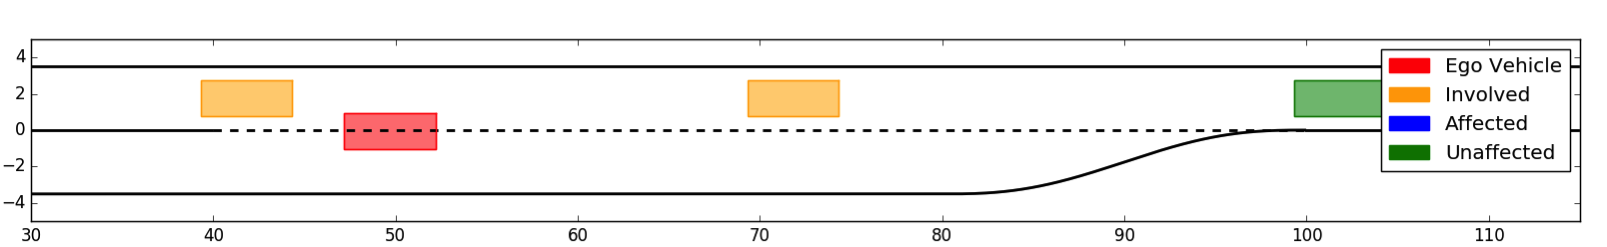
\includegraphics[width =  \textwidth]{Klassifizierung1.png}
    }
    \subfigure[]{
        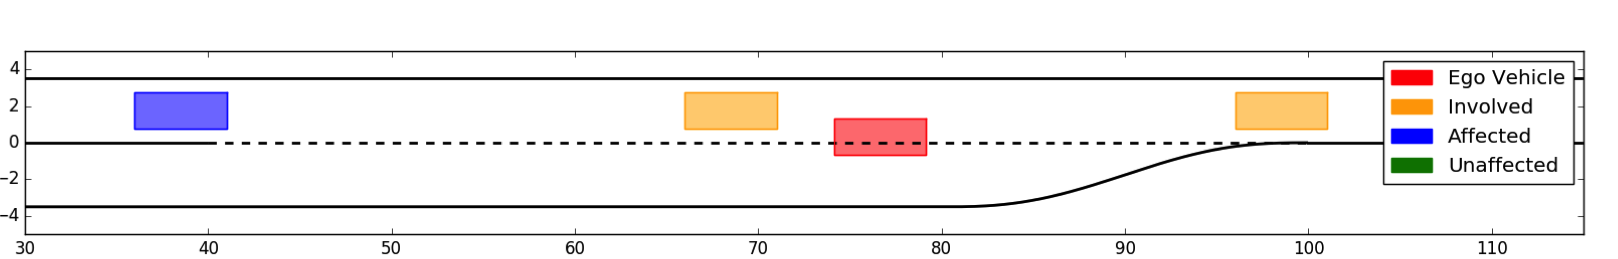
\includegraphics[width =  \textwidth]{Klassifizierung2.png}
    }
    \caption[Klassifizierung]{Klassifizierung der Fahrzeuge in der Umgebung der Ego"=Fahrzeuges (rot): beteiligte Fahrzeuge (gelb), unbeteiligte Fahrzeuge (gr\"un) und beeinflusste Fahrzeuge (blau)}
    \label{fig:Klassifizierung}
\end{figure}


Als beteiligte Fahrzeuge kommen das vorausfahrende und folgende Fahrzeug auf dem Zielfahrstreifen in Frage.
Es gilt nun zu pr\"ufen, ob die Abst\"ande zu diesen beiden Fahrzeugen auch ohne kooperatives Verhalten gro{\ss} genug sind um einen sicheren Fahrstreifenwechsel ausf\"uhren zu k\"onnen.
Daf\"ur wird nun die vom Ego"=Fahrzeug unabh\"angige Bewegungspr\"adiktion zum Zeitpunkt \gls{symb:t_lc} und die Trajektorie des Ego"=Fahrzeuges zum Zeitpunkt \gls{symb:t_lc} betrachtet.
Der Zeitpunkt \gls{symb:t_lc} wurde in Kapitel~\ref{sec:LCKostfunc} eingef\"uhrt und gibt den Zeitpunkt an, an dem das Ego"=Fahrzeug die Fahrbahnmakeriung \"uberquert.
Anhand der Bewegungspr\"adiktion und dem Zustand des Ego"=Fahrzeuges kann ermittelt werden, welches Fahrzeug sich zum Zeitpunkt \gls{symb:t_lc} vor und hinter dem Ego"=Fahrzeug auf dem Zielfahrstreifen befindet.
Ist der Abstand zum vorderen Fahrzeug bereits gr\"o{\ss}er als der geforderte Sicherheitsabstand kann davon ausgegangen werden, dass dieses kein kooperatives Verhalten zeigen wird.
Es wird als unbeteiligt eingestuft.
Ist er kleiner, so wird es als beteiligtes Fahrzeug klassifiziert.
Beim hinteren Fahrzeug muss als erstes gepr\"uft werden ob der Sicherheitsabstand zum Zeitpunkt \gls{symb:t_lc} gro{\ss} genug ist.
Ist dies der Fall muss ebenfalls gepr\"uft werden, ob es dem Fahrzeug m\"oglich ist durch eine Verz\"ogerung die geringer als \gls{symb:b_krit} ist den Sicherheitsabstand einzuhalten.
Dies muss nur gepr\"uft werden, falls die Geschwindigkeit des hinteren Fahrzeuges h\"oher ist als die des Ego"=Fahrzeuges.
In diesem Fall kann der mindestens notwendige Abstand \( d_\mathrm{nece} \) wie folgt berechnet werden:

\begin{equation}
	d_\mathrm{nece} =   T_\mathrm{abs} v_\mathrm{t,lc}^{follow} + \frac{\Delta v^2}{b_\mathrm{krit}} 
\end{equation}

Dabei ist \gls{symb:t_abs} der geforderte Zeitabstand,  \( v_\mathrm{t,lc}^{follow} \)  die Geschwindigkeit des hinteren Fahrzeuges zum Zeitpunkt \gls{symb:t_lc} und \( \Delta v \) der Geschwindigkeitsunterschied der beiden Fahrzeuge zum Zeitpunkt \gls{symb:t_lc}.
Ist der Abstand zum hinteren Fahrzeug gro{\ss} genug um diese Bedingungen zu erf\"ullen, wird davon ausgegangen, dass der Fahrstreifenwechsel ohne Kooperation stattfindet.
Das Fahrzeug wird als beeinflusst klassifiziert.
Andernfalls wird es als beteiligt eingestuft.

Die restlichen Fahrzeuge werden nun entweder als unbeteiligt oder beeinflusst eigestuft.
Fahrzeuge die sich weder auf dem aktuellen Fahrstreifen noch auf dem Zielfahrstreifen befinden werden als unbeteiligt klassifiziert.
Ebenso Fahrzeuge die sich zum Zeitpunkt \gls{symb:t_lc} vor dem Ego"=Fahrzeug befinden.
Die restlichen Fahrzeuge werden als beeinflusst eingestuft.
Die Klassifizierung der Fahrzeuge ist beispielshaft in Abbildung~\ref{fig:Klassifizierung} dargestellt.

Die Klassifzierung hat Auswirkungen darauf, wie die Fahrzeuge in den n\"achsten Schritten behandelt werden.
F\"ur beteiligte Fahrzeug wird in der inneren Optimierung ab \gls{symb:t_coop,start} bis \gls{symb:t_coop,end} eine kooperative Trajektorie ermittelt. 
Die restliche Trajektorie bis zum Ende des Planungshorizonts wird mittels dem in Kapitel~\ref{sec:IDMpred} vorgestellten \gls{idm} bestimmt.
Die unbeteiligten Fahrzeuge k\"onnen ihre urspr\"unglich ermittelte Trajektorie beibehalten.
Bei den beeinflussten Fahrzeugen wird davon ausgegangen, dass diese ab \gls{symb:t_coop,start} ihr Trajektorie anpassen m\"ussen.
F\"ur sie wird ab diesem Zeitpunkt bis zum Ende des Planungshorizonts eine neue Trajektorie anhand des \gls{idm}s bestimmt.


\subsection{Innere Optimierung}
F\"ur die als beteiligt klassifizierten Fahrzeuge soll nun die bestm\"ogliche kooperative Trajektorie gefunden werden.
Daf\"ur werden die Trajektorien im Zeitraum von \gls{symb:t_coop,start} bis \gls{symb:t_coop,end} neu bestimmt.
Werden sowohl das vordere als auch das hintere Fahrzeug auf dem Zielfahrstreifen als beteiligt klassifiziert, wird die Trajektorie zuerst f\"ur das vordere Fahrzeug ermittelt.
Anschlie{\ss}end wird auf Basis dessen die Trajektorie des folgenden Fahrzeuges ermittelt.
F\"ur jedes der Fahrzeuge wird nun ein inneres Optimierungsproblem gel\"ost.
Dabei soll die Summe aus den Kosten des beteiligten Fahrzeuges und den interaktiven Kosten des Ego"=Fahrzeuges minimiert werden.
Es ergibt sich das folgende Kostenfunktional

\begin{equation}
\label{Kostfunkin}
	G_\mathrm{lc,io} = G_\mathrm{bet,dyn} + \sum_j G_\mathrm{bet,j} + \sum_j G_\mathrm{ego,j}.
\end{equation}

\(G_\mathrm{bet,dyn}\) sind die dynamischen Kosten des beteiligten Fahrzeuges. \(G_\mathrm{bet,j}\) und \(G_\mathrm{ego,j}\) sind die Kosten des beteiligten Fahrzeuges und des Ego"=Fahrzeuges die Interaktion mit anderen Fahrzeugen entstehen.

Das Optimierungsproblem muss f\"ur den Zeitraum von \gls{symb:t_coop,start} bis \gls{symb:t_coop,end} gel\"ost werden.
Zur L\"osung dieses inneren Optimierungsproblems wurde sich erneut f\"ur ein samplingbasiertes L\"osungsverfahren entschieden.
Mit dem in Kapitel~\ref{sec:SmapPVD} vorgestellten Verfahren des Basisalgorithmus wird eine Vielzahl von Geschwindigkeitsprofilen f\"ur das beteiligte Fahrzeug erstellt.
Dabei ist der Ausgangszustand der Zustand des beteiligten Fahrzeuges zum Zeitpunkt \gls{symb:t_coop,start}.
Da der Pfad gegeben ist ergibt sich eine Vielzahl von Trajektorien.
F\"ur jede erzeugte Trajektorie werden nun die Kosten anhand des Kostenfunktionals~\ref{Kostfunkin} berechnet.
Anschlie{\ss}end wird die Trajektorie ausgew\"ahlt, die die geringsten Kosten verursacht.


\subsection{Zweifacher Fahrstreifenwechsel}
In Kapitel~\ref{sec:FrenetBesch} wird darauf eingegangen, dass ein doppelter Fahrstreifenwechsel, bei dem zwei Fahrstreifenwechsel in die gleiche Richtung ausgef\"uhrt werden, ausgeschlossen wird.
Ein Fahrstreifenwechsel auf den Zielfahrstreifen und wieder zur\"uck auf den Ausgangsfahrstreifen soll hingegen erm\"oglicht werden.
Das Wechseln auf den Zielfahrstreifen und Zur\"uckwechseln auf den Ausgangsfahrstreifen soll hier als zweifacher Fahrstreifenwechsel bezeichnet werden.
Es soll nun noch einmal genauer erl\"autert werden, warum eine Trajektorienplanung einen zweifachen Fahrstreifenwechsel erm\"oglichen sollte.
Anschlie{\ss}end wird beschrieben, wie dies in dem beschrieben Ansatz zur kooperativen Trajektorienplanung eines Fahrstreifenwechsels umgesetzt werden kann.

\begin{figure}[!htbp]
    \centering
    \subfigure[Trajektorienplanung in der die Umfahrung eines Hindernisses in zwei zeitlich versetzten Planungsschritten stattfinden muss]{
        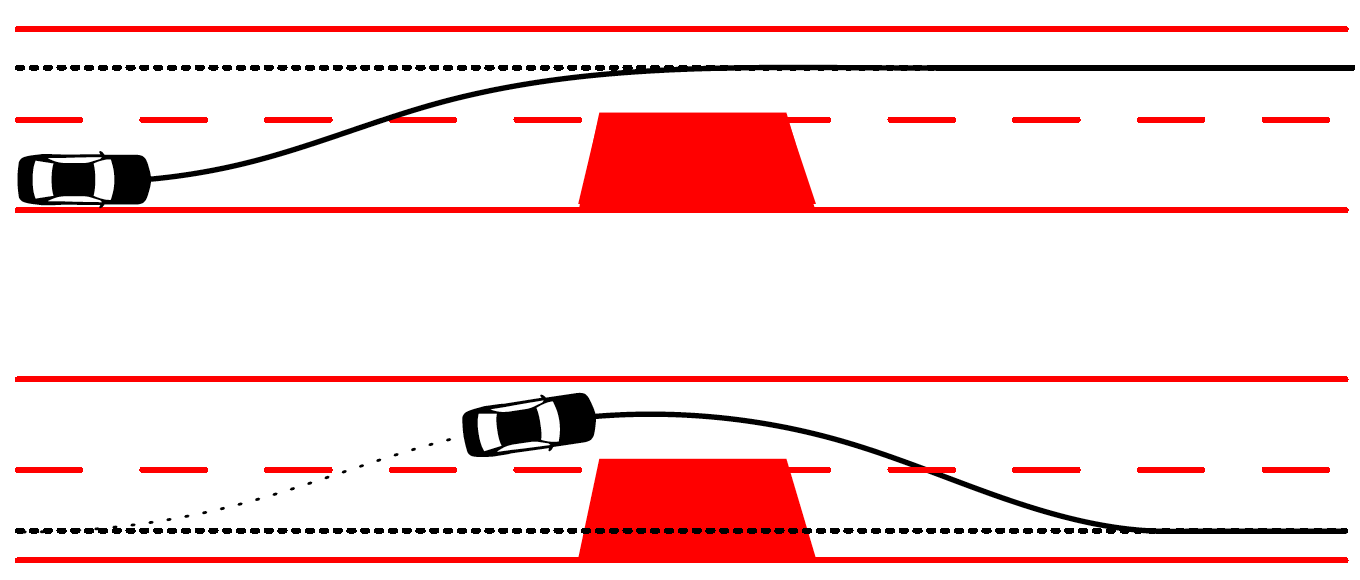
\includegraphics[width =  0.45 \textwidth]{ZweiPlanung.png}
        \label{fig:einfacherSpurw}
    }
    \hfill
    \subfigure[Trajektorienplanung in der die Umfahrung eines Hindernisses in einem Planungsschritt durchgef\"uhrt werden kann]{
        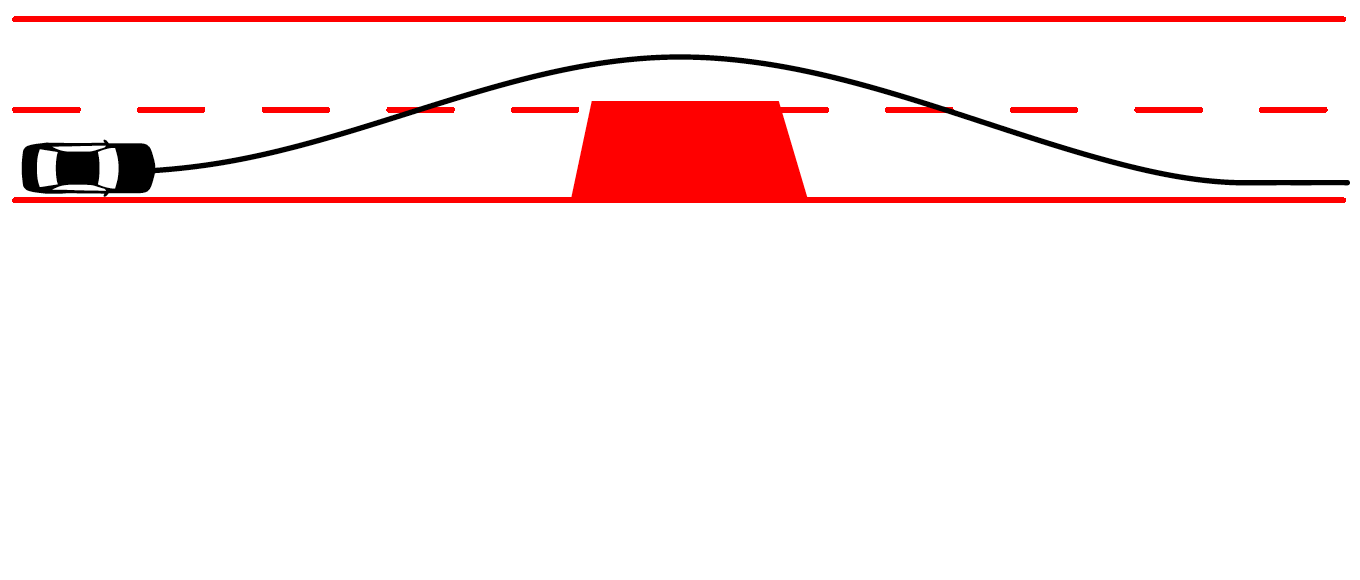
\includegraphics[width =  0.45 \textwidth]{EinPlanung.png}
        \label{fig:zweifacherSpurw}
    }
    \caption[Zweifacher Fahrstreifenwechsel]{Vergleich verschiedener Trajektorieplanungsans\"atze bei der Umfahrung eines Hindernisses \cite{Ziegler2017}}
    \label{fig:zweiSpurwech}
\end{figure}

In dem von Werling \cite{Werling2011} vorgestellten Ansatz zur Trajektorienplanung wird eine Trajektorie erzeugt, die durch ein quinitsches Polynom beschrieben wird.
Dadurch k\"onnen ruckoptimale Trajektorien generiert werden.
Ein solches Verfahren erlaubt die Planung eines einfachen Fahrstreifenwechsel in einem Planungsschritt.
Ziegler \cite{Ziegler2017} beschreibt die Suboptimalit\"at dieses Ansatzes.
Befindet sich ein Hindernis auf der Strecke wird zuerst eine Trajektorie erzeugt die dem Hindernis ausweicht (Abbildung~\ref{fig:einfacherSpurw} oben).
Erst in einem sp\"ateren Planungsschritt wird dann eine Trajektorie geplant, die wieder zur\"uck auf den Ausgangsfahrstreifen f\"uhrt (Abbildung~\ref{fig:einfacherSpurw} unten).
Eine Trajektorienplanung wie in Abbildung~\ref{fig:zweifacherSpurw} dargestellt, bei der in einem Planungsschritt sowohl das Ausweichen auf einen anderen Fahrstreifen als auch das Zur\"uckfahren auf den Ausgangsfahrstreifen geplant wird, ist nicht m\"oglich.

F\"ur das reine Umfahren eines Hindernisses ist ein Planungsansatz wie in Abbildung~\ref{fig:einfacherSpurw} dargestellt ausreichend.
Dieser Ansatz ger\"at jedoch an seine Grenzen, wenn ein \"ahnliches Man\"over bei entgegenkommenden Verkehr geplant werden soll.
Zu dem Zeitpunkt an dem der Fahrstreifenwechsel auf die Gegenspur eingeleitet wird, ist es der Trajektorienplanung noch nicht m\"oglich den Fahrstreifenwechsel zur\"uck auf den Ausgangsfahrstreifen zu planen.
Die Planung kann also vor Einleitung des Man\"overs nicht sicherstellten, dass der R\"uckwechsel ausgef\"uhrt werden kann bevor es zu einer Kollision mit dem entgegenkommendem Verkehr kommt.

Dies zeigt, dass ein Planungsverhalten wie in Abbildung~\ref{fig:zweifacherSpurw} gezeigt m\"oglich sein sollte.
In dem in Kapitel~\ref{sec:Pfadplanung} vorgestellten Teilschritt der Pfadplanung wird der Pfad f\"ur einen einfachen Fahrstreifenwechsel zu einem gegeben Geschwindigkeitsprofil erzeugt.
Erst anschlie{\ss}end wird in der inneren Optimierung und mit der Neupr\"adiktion vorherbestimmt wie die Fahrzeuge in der Umgebung des Ego"=Fahrzeuges auf diesen Fahrstreifenwechsel reagieren werden.
Die Reaktion der Fahrzeuge ist also im ersten Pfadplanungsschritt noch nicht bekannt.
Es k\"onnen deshalb in einem Pfadplanungsschritt nicht mehrere Fahrstreifenwechsel geplant werden, da der erste geplante Fahrstreifenwechsel das Verhalten der anderen Fahrzeuge beeinflusst.

F\"ur den vorliegenden Ansatz wird vorgeschlagen zun\"achst nur ein einzelnen Fahrstreifenwechsel zu planen und die Reaktion der anderen Fahrzeug auf diesen Fahrstreifenwechsel pr\"adiziert.
Ausgehend von dieser L\"osung werden dann die Schritte von der Pfadplanung bis zur Neupr\"adiktion wiederholt.
Ausgangspunkt f\"ur diesen zweiten Iterationsschritt sind die Zust\"ande der Fahrzeuge zum Zeitpunkt \gls{symb:t_coop,end}. 
Somit ist sichergestellt, dass die L\"osung der inneren Optimierung aus dem vorhergehenden Iterationsschritt erhalten bleibt.
Das Ergebnis ist ein Trajektorienset mit einer Egotrajektorie, die zwei Fahrstreifenwechsel enth\"alt.
Damit wird ein Planungsverhalten wie in Abbildung~\ref{fig:zweifacherSpurw} gezeigt erm\"oglicht.

F\"ur einen Fahrstreifenwechsel bei entgegenkommenden Verkehr ist darauf zu achten, dass hier nicht mehr der in Kapitel~\ref{sec:LCKostfunc} vorgestellte Zeitabstand \gls{symb:t_abs} verwendet werden kann.
Der Abstand zum entgegenkommenden Fahrzeug kann nicht mehr allein von der Geschwindigkeit des eigenen Fahrzeuges abh\"angig gemacht werden.
Hier sollte auf eine andere Vorgehensweise zur\"uckgegriffen werden.
Eine M\"oglichkeit bietet die Nutzung der von Naumann und Stiller \cite{Naumann2017towards} vorgestellten TZC (time of zone clearance).

\section{Fortlaufende Neuplanung}
\label{sec:Neuplanung}

Laut Hubmann et al. \cite{Hubmann2018} verursachen Unsicherheiten in der Pr\"adiktion der Trajektorie anderer Verkehrsteilnehmer eine hohe Komplexit\"at in der Trajektorieplanung.
Die Unsicherheiten ergeben sich aus:

\begin{itemize}
\item der unbekannten Route anderer Verkehrsteilnehmer,
\item den unbekannten longitudinalen Bewegungen anderer Fahrzeuge, 
\item potenziellen Interaktionen zwischen anderen Verkehrsteilnehmern und auch mit dem Ego"=Fahrzeug
\item und Ungenauigkeiten bei der Messung.
\end{itemize}

Die Ungenauigkeit in der Pr\"adiktion der Zust\"ande anderer Verkehrsteilnehmer nimmt zu, je weiter diese zeitlich vom aktuellen Zeitpunkt entfernt sind.
Je gr\"o{\ss}er die Ungenauigkeiten sind, desto schwieriger wird es f\"ur das automatisierte Fahrzeug eine sichere Trajektorie zu ermitteln.
Zus\"atzlich findet die Planung in der Regel in einem zeitlich begrenzten Horizont statt und auch die Sensoren des Fahrzeuges k\"onnen nur einen bestimmten Bereich abdecken.
Somit gelangen immer neue Bereiche der Umgebung in den Erfassungsbereich der Sensoren und es m\"ussen immer wieder neue Objekte in der Planung ber\"ucksichtigt werden.

Es ist offensichtlich, dass eine einmalige Planung, deren Trajektorie dann komplett ausgef\"uhrt wird, nicht umgesetzt werden kann.
Anstatt dessen wird bei automatisierten Fahrzeugen auf ein Vorgehen zur\"uckgegriffen, dass auch bei menschlichen Fahrern angewandt wird: die kontinuierliche Neuplanung.
Dabei wird die Planung in regelm\"a{\ss}igen Abst\"anden wiederholt.
Somit kann immer wieder auf die neue Erfassung der Umgebung reagiert werden.
Den Anfang der neu geplanten Trajektorie bildet dabei ein Teil der Trajektorie aus dem vorherigen Planungsschritt.
Damit kann eine Stetigkeit der letztendlich gefahrenen Trajektorie erreicht werden.
Das Vorgehen bei der fortlaufenden Neuplanung eines automatisierten Fahrzeuges wird von Ziegler \cite{Ziegler2017} beschrieben und ist in Abbildung~\ref{fig:Neuplanung} dargestellt.
In schwarz dargestellt ist die Trajektorie, die zum Zeitpunkt \gls{symb:t_jetzt} verf\"ugbar wurde.
Zu diesem Zeitpunkt wurde auch das rot schraffiert eingezeichnete Hindernis wahrgenommen.
Das Planungsmodul ben\"otigt maximal eine Zeit \gls{symb:t_verarb} zu Generierung der neuen Trajektorie.
Das bedeutet, dass das Fahrzeug von \gls{symb:t_jetzt} bis \gls{symb:t_jetzt} + \gls{symb:t_verarb} der schwarz eingezeichneten Trajektorie folgen muss (rot dargestellt).
Als Anfangswert zur Generierung der neuen Trajektorie wird nun der letzte Teil der alten Trajektorie aus dem Zeitbereich von \gls{symb:t_jetzt} bis \gls{symb:t_jetzt} + \gls{symb:t_verarb} genommen (blau dargestellt).
Ab \gls{symb:t_jetzt} + \gls{symb:t_verarb} wird nun die neue Trajektorie ausgef\"uhrt, die auf das erfasste Objekt reagiert und ihm ausweicht (gr\"un dargestellt).

\begin{figure}[!htbp]
    \centering
    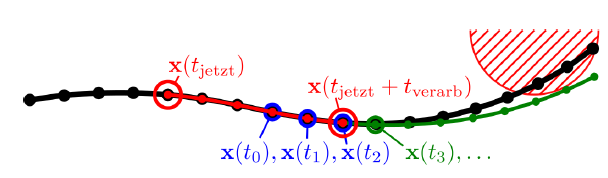
\includegraphics[width = 0.95 \textwidth]{Neuplanung.png}
    \caption[Neuplanung]{Darstellung der fortlaufenden Neuplanung \cite{Ziegler2017}}
    \label{fig:Neuplanung}
\end{figure}


Gerade in Situationen in denen es zur Interaktion mit anderen Verkehrsteilnehmern kommt ist es schwer vorherzusagen wie sich diese verhalten werden.
Eine fortlaufende Neuplanung ist somit unabdingbar.
In dem vorgestellten Ansatz wird dies umgesetzt, indem bei jedem Planungsschritt zwischen \gls{symb:t_jetzt} und \gls{symb:t_jetzt} + \gls{symb:t_verarb} der Pfad und das Geschwindigkeitsprofil der  Trajektorie aus dem vorausgegangenen Planungsschritt \"ubernommen wird.
Ab \gls{symb:t_jetzt} + \gls{symb:t_verarb} werden dann durch die zuf\"allige Generierung von R\"ucken randomisierte Geschwindigkeitsprofile erzeugt.
Alle diese Geschwindigkeitsprofile haben dadurch anf\"anglich den gleichen Verlauf.
F\"ur diese Geschwindigkeitsprofile wird dann jeweils ein Fahrstreifenwechselpfad generiert, wobei bis zum Zeitpunkt \gls{symb:t_jetzt} + \gls{symb:t_verarb} der bisherige Pfad \"ubernommen wird.

Die Trajektorien der anderen Fahrzeuge sind dem Planungsmodul unbekannt.
Im Gegensatz zum Ego"=Fahrzeug kann nicht davon ausgegangen werden, dass die anderen Fahrzeuge sich entsprechend des Ergebnisses des vorherigen Planungsschrittes verhalten werden.
Bei der Generierung der Geschwindigkeitsprofile der anderen Fahrzeuge wird als Ausgangspunkt deshalb nur der Zustand genommen der bei \gls{symb:t_jetzt} wahrgenommen wurde.
Die Geschwindigkeitsprofile werden f\"ur den gesamten Planungszeitraum neu generiert.
